% =====================================================================
%  CASA0010 MSc Dissertation
%  Compile with:  latexmk -xelatex main.tex     (or ./build.sh)
%  Body chapters are generated from ../write/*.md by md2tex.py
% =====================================================================
\documentclass[12pt,a4paper,oneside]{report}

% ---------- page geometry -------------------------------------------
\usepackage[a4paper,top=2.5cm,bottom=2.5cm,left=3cm,right=2.5cm]{geometry}

% ---------- fonts and encoding (XeLaTeX) -----------------------------
\usepackage{fontspec}
\usepackage{unicode-math}
% Referenced by filename: the TeX Live copies of these fonts are not
% registered with fontconfig on macOS, so the human-readable names fail.
\setmainfont{texgyrepagella}[
  Extension    = .otf,
  UprightFont  = *-regular,
  ItalicFont   = *-italic,
  BoldFont     = *-bold,
  BoldItalicFont = *-bolditalic,
]
\setmathfont{texgyrepagella-math.otf}
\usepackage{microtype}

% Glyphs the text uses that are safer routed through maths.
\usepackage{newunicodechar}
\newunicodechar{−}{\ensuremath{-}}
\newunicodechar{≤}{\ensuremath{\leq}}
\newunicodechar{≥}{\ensuremath{\geq}}
\newunicodechar{≈}{\ensuremath{\approx}}
\newunicodechar{≠}{\ensuremath{\neq}}
\newunicodechar{×}{\ensuremath{\times}}
\newunicodechar{±}{\ensuremath{\pm}}
\newunicodechar{÷}{\ensuremath{\div}}
\newunicodechar{ρ}{\ensuremath{\rho}}
\newunicodechar{γ}{\ensuremath{\gamma}}
\newunicodechar{Σ}{\ensuremath{\Sigma}}
\newunicodechar{∈}{\ensuremath{\in}}
\newunicodechar{→}{\ensuremath{\rightarrow}}

% ---------- spacing (handbook 4.3: generous spacing) -----------------
\usepackage{setspace}
\onehalfspacing
\usepackage{parskip}

% ---------- tables, figures, floats ----------------------------------
\usepackage{longtable,booktabs,array,calc}
\usepackage{graphicx}
\usepackage{caption}
\captionsetup{font=small,labelfont=bf,labelsep=period,skip=6pt}
\captionsetup[longtable]{skip=4pt}
\usepackage{float}
\usepackage{pdflscape}
\usepackage{adjustbox}
\usepackage{needspace}
\usepackage{etoolbox}
\makeatletter
\patchcmd\longtable{\par}{\if@noskipsec\mbox{}\fi\par}{}{}
\makeatother
% longtable zeroes \parskip and does not put it back, so every table would
% otherwise flatten the paragraph spacing for the rest of the document.
\newlength{\bodyparskip}
\newcommand{\restoreparskip}{\setlength{\parskip}{\bodyparskip}}
\apptocmd{\endlongtable}{\restoreparskip}{}{}
\usepackage{footnotehyper}
\makesavenoteenv{longtable}
\setlength{\emergencystretch}{3em}
\providecommand{\tightlist}{\setlength{\itemsep}{0pt}\setlength{\parskip}{0pt}}

% ---------- references list (hanging indent) -------------------------
\usepackage{hanging}

% ---------- headings in bold (handbook 4.3) --------------------------
\usepackage{titlesec}
\titleformat{\chapter}[display]
  {\normalfont\Large\bfseries}{\chaptertitlename\ \thechapter}{12pt}{\LARGE}
\titlespacing*{\chapter}{0pt}{0pt}{24pt}
\titleformat{\section}{\normalfont\large\bfseries}{\thesection}{1em}{}
\titleformat{\subsection}{\normalfont\normalsize\bfseries}{\thesubsection}{1em}{}

% ---------- continuous arabic pagination (handbook 4.8) --------------
\usepackage{fancyhdr}
\pagestyle{fancy}
\fancyhf{}
\fancyfoot[C]{\thepage}
\renewcommand{\headrulewidth}{0pt}
\fancypagestyle{plain}{\fancyhf{}\fancyfoot[C]{\thepage}\renewcommand{\headrulewidth}{0pt}}

% ---------- links ----------------------------------------------------
\usepackage[hidelinks,breaklinks]{hyperref}
\usepackage{xurl}
\hypersetup{
  pdftitle={Evaluating the Geographic Transfer of a US-Trained Surface-Parking Segmentation Model: Evidence from Leeds},
  pdfauthor={Jiayi Hou}
}

% =====================================================================
%  Details required on the title page by handbook 4.2
% =====================================================================
% \\ sets the break; left to itself the line turns badly
\newcommand{\thesistitle}{Evaluating the Geographic Transfer of\\a US-Trained Surface-Parking\\Segmentation Model: Evidence from Leeds}
\newcommand{\studentname}{Jiayi Hou}
\newcommand{\studentnumber}{25054106}
\newcommand{\modulecode}{CASA0010}
\newcommand{\modulename}{MSc Urban Spatial Science Dissertation}
% ~ binds the second name so the line breaks after "and", not mid-name.
\newcommand{\supervisors}{Associate Professor Esra Suel and Dr~Clara~Peiret-Garc\'ia}
\newcommand{\submissiondate}{August 2026}
\newcommand{\repourl}{https://github.com/hou1020/Parking}
\newcommand{\wordcount}{11{,}953}

\begin{document}
% \baselineskip is not yet set in the preamble, so the paragraph gap has to
% be fixed here, once \onehalfspacing is in force.
\setlength{\bodyparskip}{0.5\baselineskip}
\setlength{\parskip}{\bodyparskip}
\pagenumbering{arabic}

% =====================================================================
%  Title page
% =====================================================================
{\centering
\vspace*{1cm}

{\LARGE\bfseries\begin{tabular}{c}\thesistitle\end{tabular}\par}

\vspace{2.4cm}
{\large \studentname\par}
\vspace{0.4cm}
{\large \submissiondate\par}

\vspace{2.2cm}
\begin{minipage}{0.85\textwidth}
\centering
\small
\begin{tabular}{@{}r@{\hspace{1.2em}}>{\raggedright\arraybackslash}p{0.66\textwidth}@{}}
\textbf{Student number} & \studentnumber \\
\textbf{Module} & \modulename \\
\textbf{Module code} & \modulecode \\
\textbf{Supervisors} & \supervisors \\
\textbf{Code repository} & \url{\repourl} \\
\textbf{Word count} & \wordcount \\
\end{tabular}
\end{minipage}

\vfill
\begin{minipage}{0.85\textwidth}
\centering\small
This dissertation is submitted in part requirement for the MSc in the Centre
for Advanced Spatial Analysis, Bartlett Faculty of the Built Environment, UCL.
\end{minipage}
\vspace{1cm}
\par}
\clearpage

% =====================================================================
%  Abstract  (handbook 4.2: max 300 words, not counted)
% =====================================================================
\chapter*{Abstract}
\addcontentsline{toc}{chapter}{Abstract}
\input{chapters/00_abstract}

% =====================================================================
%  Declaration  (handbook 4.2, wording fixed)
% =====================================================================
\chapter*{Declaration}
\addcontentsline{toc}{chapter}{Declaration}

I hereby declare that this dissertation is all my own original work and that
all sources have been acknowledged. It is \wordcount{} words in length.

\vspace{1.5\baselineskip}

\noindent
\begin{tabular}{@{}l@{\hspace{1em}}l@{}}
Signed: & \hspace*{5cm} \\[1.2em]
Date:   & 20 August 2026 \\
\end{tabular}

% =====================================================================
%  Acknowledgements
% =====================================================================
\chapter*{Acknowledgements}
\addcontentsline{toc}{chapter}{Acknowledgements}

I thank my supervisors, Associate Professor Esra Suel and Dr Clara
Peiret-Garc\'ia, for their guidance and for their patience with a project that
changed shape more than once.

At the Centre for Cities, I thank Maurice Lange, who set the question in its
policy context, arranged for me to work from the office, and gave advice
throughout.

I am also grateful to Shirin Qiam, Saipraneeth Devunuri and Lewis Lehe, whose
released model and pipeline this study is built on.

% =====================================================================
%  Contents and lists
% =====================================================================
\cleardoublepage
\phantomsection
\addcontentsline{toc}{chapter}{Contents}
\tableofcontents

\cleardoublepage
\phantomsection
\addcontentsline{toc}{chapter}{List of Figures}
\listoffigures

\cleardoublepage
\phantomsection
\addcontentsline{toc}{chapter}{List of Tables}
\listoftables

% =====================================================================
%  Acronyms and abbreviations  (handbook 4.2)
% =====================================================================
\chapter*{Acronyms and Abbreviations}
\addcontentsline{toc}{chapter}{Acronyms and Abbreviations}

\begin{tabular}{@{}p{3.2cm}p{\dimexpr\textwidth-3.6cm\relax}@{}}
\toprule
CASA & Centre for Advanced Spatial Analysis, UCL \\
FN & False negative --- labelled parking the model did not predict \\
FP & False positive --- predicted parking that is not labelled parking \\
GSD & Ground sample distance \\
IoU & Intersection over union \\
MHCLG & Ministry of Housing, Communities and Local Government \\
NIR & Near infrared \\
NPPF & National Planning Policy Framework \\
OS & Ordnance Survey \\
OSM & OpenStreetMap \\
RQ & Research question \\
TP & True positive --- predicted parking that is labelled parking \\
VOA & Valuation Office Agency \\
\bottomrule
\end{tabular}

% =====================================================================
%  Body
% =====================================================================
\chapter{Introduction}\input{chapters/01_introduction}
\chapter{Literature Review}\input{chapters/02_background}
\chapter{Methodology}This chapter sets out how the transfer was tested. It describes the study area and the imagery the model consumed (§3.1), the annotation protocol used to build an independent reference (§3.2), the segmentation pipeline itself (§3.3), and the accuracy measures (§3.4). It then sets out the two complementary procedures used to characterise error --- automated attribution against reference layers (§3.5) and stratified sampling with visual adjudication (§3.6) --- followed by the ablation design used to isolate the contribution of building and road subtraction (§3.7). Two checks close the chapter: one on the imagery underlying the reference and the predictions (§3.8), and one on the estimator used to correct the model's systematic bias (§3.9).

\hypertarget{study-area-and-data}{%
\section{Study area and data}\label{study-area-and-data}}

The study area is a 100 km² square centred on Leeds, divided into one hundred 1 km² cells on the British National Grid (Figure 3.1). The city centre is taken as City Square (E 429832, N 433449); cell centroids lie between 0.34 km and 7.64 km from it. Leeds was chosen as a large English city outside London with substantial surface parking in and around its core, and with complete aerial coverage at the resolution the model requires. The choice also aligns with the project's Centre for Cities framing: Leeds is among the large British cities the organisation identifies as having some of the largest density gaps relative to their international peers (Lange, Kovacevic and Johnson, 2026). A square grid rather than an administrative boundary was used so that every cell is an equal-area unit and per-cell statistics are directly comparable. The choice of areal unit is not neutral --- figures computed over zones depend on how the zones are drawn, the modifiable areal unit problem (Openshaw,
1984) --- so the unit is held constant throughout and whole-area figures are reported alongside per-cell ones.

\begin{figure}[htbp]
\centering
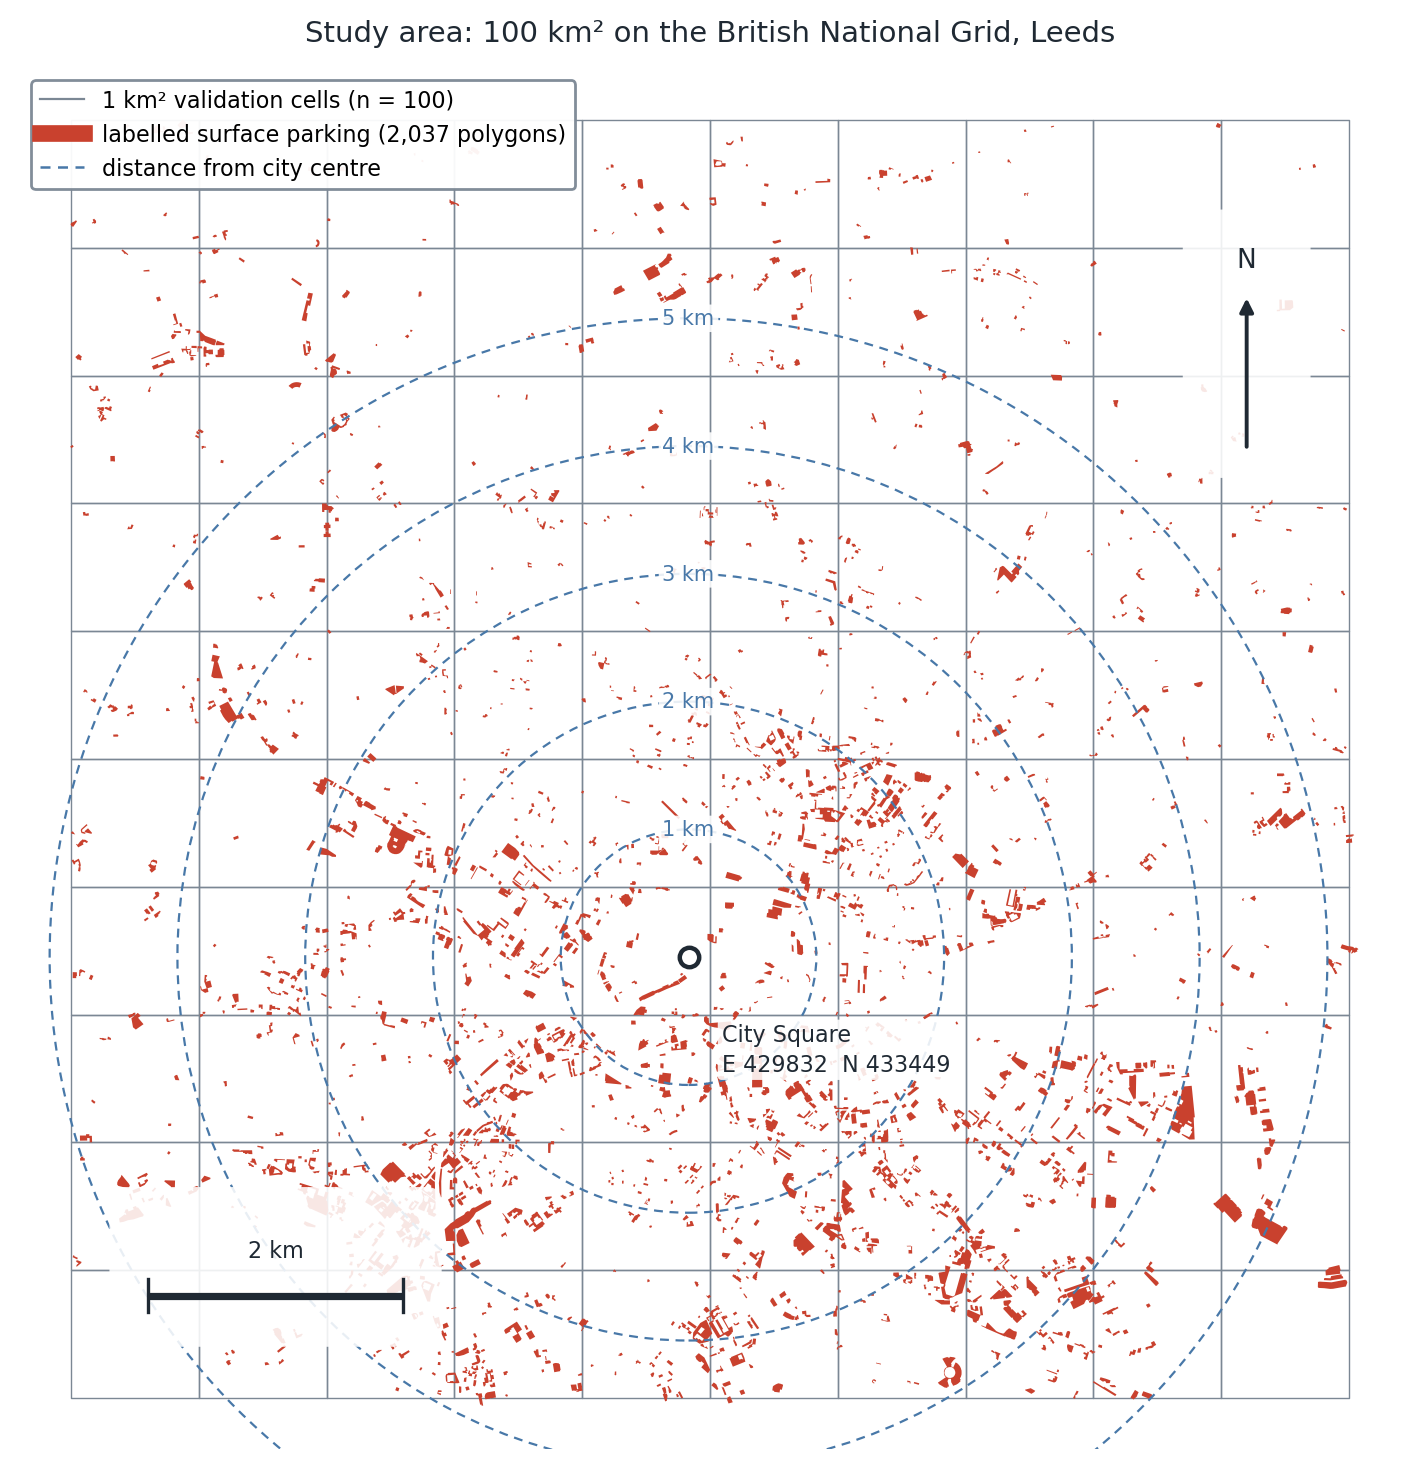
\includegraphics[width=\linewidth,height=0.82\textheight,keepaspectratio]{figures/fig_study_area.png}
\caption{The study area: one hundred 1 km² validation cells on the British National Grid, the 2,037 manually labelled surface parking polygons, and distance rings from City Square. Labelled parking is visibly concentrated in a band around, rather than at, the centre --- a pattern quantified in §4.7.}
\label{fig:3.1}
\end{figure}\restoreparskip

The imagery is Getmapping aerial photography supplied through Digimap: 100 tiles at 0.25 m ground sample distance, three visible bands (RGB), projected in EPSG:27700. All spatial operations are carried out in EPSG:27700, whose units are metres, so polygon areas are read directly in m² without further projection.

Three reference datasets are used, none of them as ground truth. OpenStreetMap building footprints and road centrelines (retrieved 25 June 2026) are inputs to the post-processing stage. OpenStreetMap land use, brownfield, pitch and \texttt{amenity=parking} polygons are used only to attribute errors after the fact. Ordnance Survey Open Greenspace supplies sports facilities. The distinction matters: reference layers are used here to explain where errors fall, and --- with the deliberate exception tested in §3.7 --- never to decide what the map should contain.

Appendix D lists the code repository, the licensing position of each dataset and the file behind every table reported here. The manual reference labels are available in the repository, but the institutionally licensed aerial imagery cannot be redistributed.

\hypertarget{annotation-protocol}{%
\section{Annotation protocol}\label{annotation-protocol}}

Accuracy figures are only meaningful against a reference that follows the definition the model was trained on. The annotation rules therefore follow those of Qiam, Devunuri and Lehe (2025), whose dataset the model was trained on, and are reproduced in full in Appendix A. The target is off-street surface parking: open-air parking surfaces visible from above, outside the public road. Labels are binary. No minimum size threshold is applied. Marked bays and the aisles connecting them are included, as is rooftop parking where the parking surface is visible from above; on-street parking and enclosed multi-storey structures are excluded. Where markings are absent, an area is labelled only where parked vehicles and a bay-and-aisle layout together make the use unambiguous. Boundaries are drawn at the edge of the paving rather than the parcel line.

One boundary inside residential parking is worth stating explicitly, because it is the commonest ambiguous case in a British city. Parking courts shared between several dwellings are labelled; driveways and forecourts serving a single household are not. A communal court resembles a small car park in layout and in what it does, while a single driveway does not. The distinction is not introduced here: UK parking measurement already separates private residential parking into driveway and communal categories, and the two were surveyed and reported separately in the London study described in §2.2 (Bates and Leibling, 2012).

Labelling was carried out in QGIS by a single annotator over a satellite basemap, producing 2,037 polygons with a confidence attribute (3 = clear, 2 = fairly clear, 1 = uncertain) and a free-text note used to flag rooftop cases. Summed individually the polygons cover 3.2677 km². Dissolving them leaves both the area and the part count unchanged, so no two labelled polygons overlap; the reference is nonetheless dissolved before every comparison, since the accuracy measures of §3.4 are only well defined on non-overlapping geometry and the property should be enforced rather than assumed. Clipping to the study grid removes 0.0081 km² where polygons cross the outer boundary, giving the 3.2597 km² used throughout. One cell (c0r9) contains no labelled parking, so recall is undefined there and per-cell statistics involving recall use \(n = 99\).

Single-annotator labelling remains a limitation, taken up in §5.5.

\hypertarget{model-and-pipeline}{%
\section{Model and pipeline}\label{model-and-pipeline}}

The model is the SegFormer (Xie et al., 2021) parking-lot segmentation network released by Qiam, Devunuri and Lehe (2025). The released checkpoint is a B5 configuration whose backbone was initialised from Cityscapes weights and fine-tuned by those authors on their parking dataset, as documented in the released model card and repository. In the primary analysis, its weights are used exactly as released: no UK imagery is used to update them. The network is therefore evaluated under zero-shot geographic transfer, although the surrounding pipeline includes the UK-specific tiling and post-processing described below and isolated by the ablation in §3.7. Appendix C reports a separate experiment on a fixed 40/10/50 cell split, comparing generic fine-tuning, positional targeted loss weighting and validation-selected thresholding on raw-pixel outputs without post-processing. Those results remain separate from the primary analysis in §§4.1--4.7.

\begin{figure}[htbp]
\centering
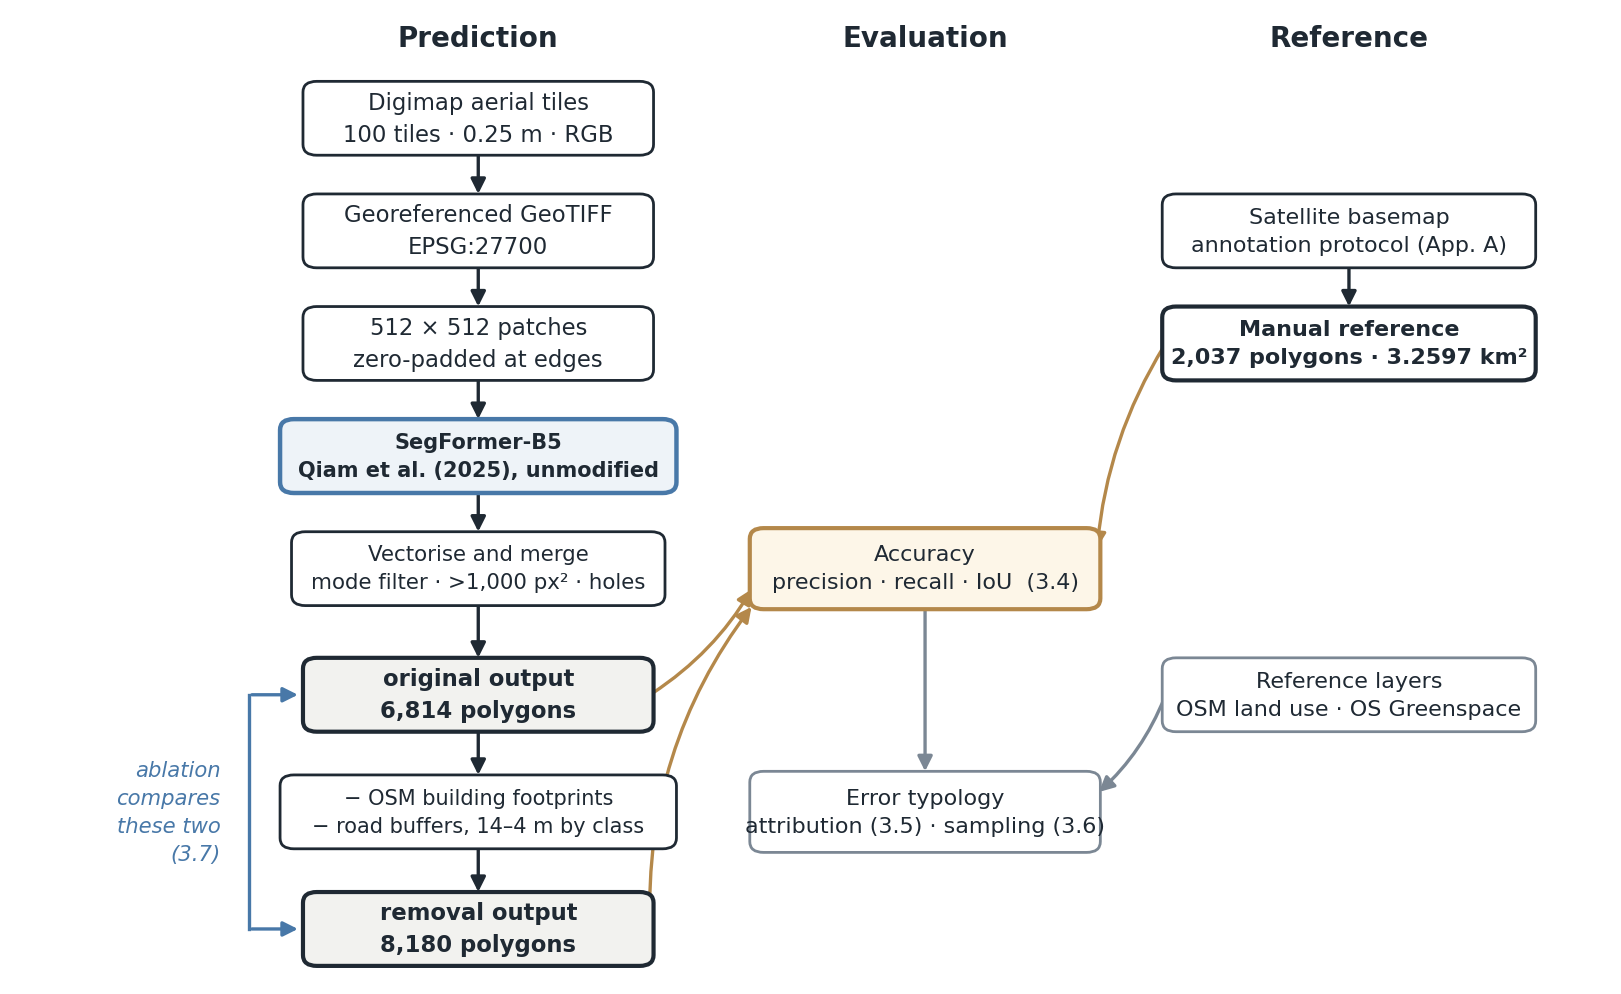
\includegraphics[width=\linewidth,height=0.82\textheight,keepaspectratio]{figures/fig_pipeline.png}
\caption{The processing chain. Prediction runs from Digimap tile to outputs before and after building and road subtraction, which the ablation of §3.7 compares. The manual reference and the model outputs meet at the accuracy measures of §3.4; the reference layers enter only at the error-attribution stage of §§3.5--3.6.}
\label{fig:3.2}
\end{figure}\restoreparskip

The pipeline proceeds in five stages. Digimap tiles and their world files are converted to georeferenced GeoTIFFs. Each tile is cut into 512 × 512 pixel patches, zero-padded at the edges. Patches are passed through the network and the upsampled logits reduced to a binary mask by argmax. Masks are cleaned with a mode filter and vectorised by contour extraction, with components below 1,000 px² (about 62 m² at 0.25 m) discarded and enclosed holes subtracted; polygons are then transformed from pixel to grid coordinates and merged across tiles.

Two post-processing subtractions follow, both UK adaptations of operations already present in the released pipeline, which likewise subtracts building footprints and buffered OpenStreetMap roads (Qiam, Devunuri and Lehe, 2025). Here, OpenStreetMap building footprints replace the source pipeline's Microsoft US building data and are subtracted under its premise that roofs are false positives --- a premise tested against rooftop parking in §3.7. Road centrelines are buffered by carriageway class (Table 3.1), rather than by recorded lane count alone, dissolved, and subtracted.

\begin{table}[htbp]
\centering
\caption{Road buffer half-widths by OSM \texttt{highway} class. Where a \texttt{lanes} tag is present, the width is the greater of the tabulated value and 3 m per lane.}\label{tab:3.1}
\begin{adjustbox}{max width=\textwidth}
\begin{tabular}{@{}lrllr@{}}
\toprule
Class & Width (m) & & Class & Width (m) \\
\midrule
motorway & 14 & & tertiary & 7 \\
trunk & 12 & & tertiary\_\allowbreak{}link & 5 \\
primary & 10 & & unclassified & 5 \\
secondary & 8 & & residential & 5 \\
motorway\_\allowbreak{}link & 9 & & living\_\allowbreak{}street & 4 \\
trunk\_\allowbreak{}link & 8 & & \emph{default} & \emph{5} \\
primary\_\allowbreak{}link & 7 & & & \\
secondary\_\allowbreak{}link & 6 & & & \\
\bottomrule
\end{tabular}
\end{adjustbox}
\end{table}
\restoreparskip

The half-widths are approximations by class rather than measured carriageway dimensions: each value is a plausible half-width for the road type the OSM class denotes, with 5 m applied to any class not listed. Footways, cycleways, bridleways, tracks, steps, pedestrian ways and service roads, among others, are excluded from the road layer, service roads in particular because they commonly run \emph{through} car parks; buffering them would remove the aisles the protocol explicitly includes. Both subtractions are evaluated rather than assumed in §3.7.

The output before subtraction (6,814 polygons) and after (8,180 polygons) are both retained. The increase in count reflects single lots being split by the subtracted geometry, which is why polygon counts are never interpreted as numbers of car parks.

\hypertarget{validation-design}{%
\section{Validation design}\label{validation-design}}

Accuracy is measured by area rather than by object, following the general practice in land-cover accuracy assessment of comparing a map against an independent reference over a defined spatial support (Foody, 2002; Olofsson et al., 2014). Let \(M\) and \(R\) denote the dissolved model and reference geometry, and \(|\cdot|\) denote area in m². Dissolving before comparison ensures overlapping geometry is not double-counted. The three quantities are then set operations:

\[
\mathrm{TP} = M \cap R, \qquad \mathrm{FP} = M \setminus R, \qquad \mathrm{FN} = R \setminus M
\]

from which

\[
\text{precision} = \frac{|\mathrm{TP}|}{|\mathrm{TP}| + |\mathrm{FP}|}, \qquad
\text{recall} = \frac{|\mathrm{TP}|}{|\mathrm{TP}| + |\mathrm{FN}|}, \qquad
\text{IoU} = \frac{|\mathrm{TP}|}{|\mathrm{TP}| + |\mathrm{FP}| + |\mathrm{FN}|}
\]

Area-based measures were chosen because the study asks how much land the map assigns to parking. Object-based matching would require an arbitrary rule for deciding whether split or merged polygons represent the same lot, particularly after post-processing. Since accuracy estimates depend on the assessment unit, the unit should reflect the intended use of the map (Stehman and Wickham, 2011; Stehman and Foody, 2019). As an internal check, \(|M| = |\mathrm{TP}| + |\mathrm{FP}|\) and \(|R| = |\mathrm{TP}| + |\mathrm{FN}|\); both hold to four decimal places.

Two aggregations over the \(n\) cells are reported. Writing \(\mathrm{TP}_c\) for the true positive area within cell \(c\), the micro (area-weighted) and macro (cell-averaged) forms of precision are

\[
p_{\text{micro}} = \frac{\sum_c |\mathrm{TP}_c|}{\sum_c\left(|\mathrm{TP}_c| + |\mathrm{FP}_c|\right)},
\qquad
p_{\text{macro}} = \frac{1}{n}\sum_c \frac{|\mathrm{TP}_c|}{|\mathrm{TP}_c| + |\mathrm{FP}_c|}
\]

and recall and IoU follow the same pattern. The terms are borrowed from classification evaluation, where the same two averages are taken over classes; here they are taken over spatial units. The micro figure treats the whole study area as one unit, so large car parks carry proportionate weight; it answers whether the \emph{total area} is right, and because summing over cells returns the whole-area quantity, it does not depend on how the cells were drawn. The macro figure weights every cell equally regardless of how much parking it contains, and does depend on it. The two are reported side by side because a global figure summarises the map as a whole while masking how accuracy varies across it, and local accuracy is better reported as an accompaniment to the global figure than in place of it (Foody, 2005; Stehman and Foody, 2019). Doing so needs a reference dense enough to support a figure in every sub-region, ordinarily the obstacle to it; here the reference is wall-to-wall rather than
sampled, so every cell carries its own. Macro is used as a diagnostic of uniformity rather than as an estimator of any population quantity, and the difference between the two is itself the result: where macro falls below micro, the model is performing worse in cells with little parking than the area-weighted figure suggests.

\hypertarget{error-typology-i-automated-attribution}{%
\section{Error typology I: automated attribution}\label{error-typology-i-automated-attribution}}

The first characterisation of error asks where FP and FN area falls relative to independent layers. It is applied exhaustively to all of it.

\textbf{Boundary effects are separated first.} Area-based measures cannot distinguish a slightly oversized car park from a false detection elsewhere when the error area is the same (Csurka, Larlus and Perronnin, 2013). Boundary IoU restores sensitivity to such errors by evaluating within a fixed contour band, particularly for large objects whose interiors dominate Mask IoU (Cheng et al., 2021). This study adapts that principle to partition, rather than rescore, boundary and non-boundary error.

FP area within a fixed distance \(d\) of a labelled lot is boundary \emph{dilation} --- the model drawing the same car park slightly too large --- as distinct from a standalone false detection elsewhere. Symmetrically, FN area within \(d\) of a predicted area is \emph{erosion}: reference area the model did not cover, but lying immediately alongside something it did find.

\[
\mathrm{FP}_{\text{dilation}}(d) = \mathrm{FP} \cap \big(R \oplus d\big), \qquad
\mathrm{FN}_{\text{erosion}}(d) = \mathrm{FN} \cap \big(M \oplus d\big)
\]

where \(\oplus\) denotes dilation by a buffer of \(d\) metres. Erosion is defined against the \emph{prediction} rather than against the reference boundary, so that it captures only reference area adjacent to a detection; defining it against the reference boundary would also count the outer edge of lots the model missed entirely, which is a detection failure rather than a boundary effect. Because no threshold separates the two cleanly, results are reported at \(d = 2\), 5 and 10 m, with 5 m used as the working value. Sensitivity to the width chosen is a known property of band-based measures rather than a peculiarity of this application (Cheng et al., 2021), which is why three are given. That 5 m is a convention rather than a natural break is also visible in the sampled evidence: the three sampled FP fragments that no category explained sit at a median distance of exactly 5.0 m from the nearest labelled lot, against 30.4--168.6 m across the substantive categories.

\textbf{Standalone FP is then attributed in two ways, reported side by side.}

\begin{itemize}
\tightlist
\item
  An exclusive partition: reference layers \(L_1,\dots,L_k\) are peeled off in sequence, each claiming only the area not already claimed, so shares sum to 100\%. Layers are ordered by how precisely they locate the phenomenon --- building footprints and sports pitches, which are exact polygons, before road proximity buffers, before broad land-use classes --- with industrial and commercial land last because it is the least specific evidence.
\item
  An unordered overlap: each layer is intersected with all FP independently, \(\mathrm{FP} \cap L_j\), so categories may overlap one another and need not sum to 100\%.
\end{itemize}

Presenting both means the substantive conclusions do not depend on the chosen ordering; as a robustness check, moving industrial land from an early position to last changes its exclusive share from 30.0\% to 29.6\%. The two have different denominators and are not differences of one another --- a point carried into the results tables, where the exclusive column includes the dilation band as its first row so that it sums to 100\%.

\textbf{FN is defined at the level of the car park, not the fragment.} An earlier version defined missed parking as reference area more than 5 m from any prediction, which conflated genuinely undetected car parks with the ragged edges of ones the model had largely found. Two diagnostics showed this: of 297 such fragments, 221 lay at a distance of exactly 5.0 m --- the threshold itself --- and 19.2\% of the area belonged to lots the model had detected to better than 70\%. FN is therefore partitioned by the \emph{coverage} of the lot it belongs to, \(\gamma = |R_i \cap M| / |R_i|\):

\begin{table}[htbp]
\centering
\begin{adjustbox}{max width=\textwidth}
\begin{tabular}{@{}lll@{}}
\toprule
Class & Coverage & Treatment \\
\midrule
whole lot missed & \(\gamma \le 0.10\) & a detection failure \\
partly detected & \(0.10 < \gamma \le 0.70\) & partial failure \\
fringe of detected lot & \(\gamma > 0.70\) & boundary imprecision \\
\bottomrule
\end{tabular}
\end{adjustbox}
\end{table}
\restoreparskip

Both cut points are conventions, as the 5 m band is, and both were varied. The lower one is not load-bearing: from \(\gamma \le 0.05\) to \(\gamma \le 0.20\) the whole-lot-missed share moves between 22.3\% and 29.9\% of FN, and the unresolved whole-lot remainder between 2.0\% and 2.9\% of labelled area, so what is concluded from it does not turn on where it sits. The upper one is more consequential --- at 0.60, 0.70 and 0.80 the fringe class takes 51.0\%, 44.4\% and 31.9\% of FN --- so that share is quoted with its threshold attached.

Only the first is treated as a detection failure, and is further attributed to subtraction-stage removal, rooftop labelling, containment within OSM buildings, or left unresolved.

Throughout, attribution is positional and is worded as such. A false positive lying on OSM industrial land is reported as \emph{located on} industrial land; it is not a claim that each such polygon was individually confirmed to be a storage yard.

\hypertarget{error-typology-ii-stratified-sampling}{%
\section{Error typology II: stratified sampling}\label{error-typology-ii-stratified-sampling}}

Automated attribution leaves a residual in each direction that no reference layer explains. These residuals are characterised by stratified random sampling with visual adjudication (Table 3.2). The design follows the three-part structure recommended for accuracy assessment --- a sampling design, a response design specifying how each sampled unit is judged, and an analysis that scales the sample back to the population (Olofsson et al., 2014; Stehman and Foody, 2019).

\begin{table}[htbp]
\centering
\caption{Sampling design. Large polygons are deliberately oversampled; the ratio estimator corrects for this.}\label{tab:3.2}
\begin{adjustbox}{max width=\textwidth}
\begin{tabular}{@{}llrrr@{}}
\toprule
Population & Stratum (m²) & Polygons & Area (km²) & Sampled \\
\midrule
Unexplained FP & 100--300 & 604 & 0.1055 & 20 \\
& 300--1,000 & 327 & 0.1656 & 25 \\
& \textgreater{} 1,000 & 61 & 0.1172 & 25 \\
Whole lots missed & 100--300 & 34 & 0.0079 & 10 \\
& 300--1,000 & 51 & 0.0292 & 15 \\
& \textgreater{} 1,000 & 17 & 0.0377 & 17 \\
OSM-only parking & 100--300 & 97 & 0.0192 & 5 \\
& 300--1,000 & 117 & 0.0625 & 10 \\
& \textgreater{} 1,000 & 59 & 0.1793 & 15 \\
\textbf{Total} & & & & \textbf{142} \\
\bottomrule
\end{tabular}
\end{adjustbox}
\end{table}
\restoreparskip

Estimates use a stratified ratio estimator (Cochran, 1977). For stratum \(h\) of known total area \(A_h\), with sample \(s_h\) and polygon areas \(a_i\), the estimated area of category \(c\) is

\[
\hat{A}_c = \sum_h A_h \cdot \frac{\sum_{i \in s_h,\, i \in c} a_i}{\sum_{i \in s_h} a_i}
\]

so that oversampling of large polygons does not distort the totals. Intervals on these estimates come from a stratified bootstrap: the inspected polygons are resampled with replacement within each stratum and the estimator recomputed 5,000 times, with each replicate's deviation scaled by \(\sqrt{1 - n_h/N_h}\) so that heavily sampled strata contribute proportionately less spread --- the largest missed-lot stratum, inspected in full at 17 of 17, contributes none. The intervals cover sampling variance only: not adjudication error, and not the frame exclusion described next.

The sampling frame excludes polygons below 100 m². For unexplained FP this removes 0.0513 km², or 11.7\% of that population (0.4396 km² in total, 0.3883 km² in frame). Percentages reported for this population are therefore shares of the frame, and the corrections derived from them (§4.6) implicitly assume the excluded slivers have the same composition as the sampled material. The assumption is conservative in the direction that matters: were the slivers composed like the sampled polygons, the upward correction to precision would be \emph{larger} than the one reported. Slivers below 100 m² are in any case more plausibly boundary artefacts than real parking, so they are not extrapolated to.

Each sample was inspected as an image chip cut from the Digimap tiles and assigned one category from a fixed list, with an optional note. Adjudication was carried out against the Digimap imagery, since a model's failure can only be assessed against the imagery it was given. Categories are organised by failure \emph{mechanism} rather than surface appearance --- what visual cue was absent --- so that the typology maps onto plausible causes rather than onto descriptions.

\hypertarget{ablation-design}{%
\section{Ablation design}\label{ablation-design}}

The contribution of each building and road subtraction is measured by a \(2 \times 2\) factorial design: the pre-subtraction prediction, buildings removed only, roads removed only, and both. Because set difference is commutative in the relevant sense,

\[
(X \setminus A) \setminus B = X \setminus (A \cup B)
\]

order does not affect this design; order matters only for the exclusive partition of §3.5. As a check that the reconstruction is faithful, applying both subtractions in one operation is compared against the pipeline's own tile-by-tile output; the two agree on all three reported measures to the displayed precision, so the ablation can be trusted to isolate these two operations.

A second set of variants tests the reference layers as filters rather than as explanations. Sports pitches, industrial and commercial land, and road buffers widened by a further 6 m are each subtracted from the finished map, singly and together. This is a deliberate test of a tempting inference: a layer that explains where errors fall might be assumed to improve the map if used to remove them. Reporting recall alongside precision for these variants is what makes the test informative.

Rooftop parking is examined separately as a case where the pipeline and the model can be shown to disagree. The sixteen labelled rooftop lots are compared against both the pre-subtraction and post-subtraction outputs.

\hypertarget{consistency-of-the-two-imagery-sources}{%
\section{Consistency of the two imagery sources}\label{consistency-of-the-two-imagery-sources}}

Labelling was carried out over a satellite basemap, whereas the model operated on Digimap aerial tiles. Differences between the sources could therefore contribute to the measured error. One spatial diagnostic and two checks of reference--imagery disagreement assess that contribution.

\textbf{(i) Spatial alignment.} For the 1,478 labelled lots larger than 300 m² and covered by the model by at least 70\%, let \(\mathbf{d}_i\) be the vector from the centroid of the labelled polygon to the centroid of the predicted area within it. A common directional displacement makes the mean vector large relative to the average displacement magnitude, whereas varying boundary errors tend to cancel. The ratio is

\[
\rho = \frac{\left\lVert \bar{\mathbf{d}} \right\rVert}{\frac{1}{n}\sum_i \lVert \mathbf{d}_i \rVert},
\qquad \bar{\mathbf{d}} = \frac{1}{n}\sum_i \mathbf{d}_i
\]

with \(\rho \to 0\) where the common directional component is small relative to the scatter, and \(\rho \to 1\) where displacement vectors share a common direction. Here \(\lVert\bar{\mathbf{d}}\rVert = 0.208\) m (0.83 pixels at 0.25 m resolution), against a mean displacement magnitude of 1.247 m (4.99 px), giving \(\rho = 0.167\). Non-zero mean components and a non-uniform direction distribution are statistically detectable (\(p < 0.001\)), but with 1,478 lots the sub-pixel magnitude is more informative than significance. This diagnostic shows no large common directional displacement among well-detected lots, so gross misregistration is unlikely to dominate the measured boundary error.

\textbf{(ii) An unresolved residual.} The whole-lot FN attribution in §3.5 leaves 0.0699 km² unresolved after separating areas associated with post-processing removal, rooftop labels and containment within building footprints. This is 2.1\% of labelled area. If the entire residual were treated as reference--imagery disagreement, recall would rise from 0.854 to 0.873. This is a sensitivity scenario for the unresolved residual, not a strict upper bound on all disagreement between the sources.

\textbf{(iii) A sampled estimate.} The stratified sample in §3.6 covers whole labelled lots with no more than 10\% coverage in both the post- and pre-subtraction outputs, excluding tagged rooftops and polygons below 100 m²; its frame contains 0.0748 km² of labelled lot area. Adjudication against the model's input imagery estimates 0.0313 km², or 1.0\% of labelled area, as not parking in that imagery. In the reference-side correction used here, removing it raises recall from 0.854 to 0.863 and leaves precision unchanged.

Separately, last-edit timestamps were retrieved for all 985 OSM parking features to test whether OSM disagreement simply reflects stale records. The 11 sampled features with no parking visible in the imagery had a median last-edit year of 2025, the most recent of any sampled category. This does not support stale OSM records as a general explanation; timestamps record any edit, including tag-only changes, rather than construction.

\hypertarget{the-calibration-estimator-and-its-spatial-grain}{%
\section{The calibration estimator and its spatial grain}\label{the-calibration-estimator-and-its-spatial-grain}}

Adjusting mapped area for commission and omission error using reference data is established practice (Olofsson et al., 2014). Here, where a map has precision \(p\) and recall \(r\), predicted area \(|M|\) relates to reference area \(|R|\) by

\[
|M| \cdot p = |\mathrm{TP}| = |R| \cdot r
\qquad\Longrightarrow\qquad
|R| = |M| \cdot \frac{p}{r}
\]

Applied to the same cells used to measure \(p\) and \(r\), this is an identity rather than an independent estimate. The factor simplifies to an area ratio:

\[
\frac{p}{r} = \frac{|\mathrm{TP}|/|M|}{|\mathrm{TP}|/|R|} = \frac{|R|}{|M|}
\]

Fitting it therefore requires only labelled and predicted total area over the calibration cells, not an object-level error analysis. Its usefulness must be tested on cells not used to fit it.

Three hold-out schemes test whether a factor fitted on one part of the city predicts another, and at what grain (Table 3.3). Each fits \(p/r\) on cells \(\mathcal{T}\) and applies it to held-out cells \(\mathcal{H}\). Whole cells, rather than polygons, are withheld because short-range spatial dependence means that randomly splitting dependent units can understate predictive error (Roberts et al., 2017). Error is reported relative to labelled area in the held-out set:

\[
e = \frac{\left(\sum_{c \in \mathcal{H}} |M_c|\right)\left(p/r\right)_{\mathcal{T}} - \sum_{c \in \mathcal{H}} |R_c|}{\sum_{c \in \mathcal{H}} |R_c|}
\]

\begin{table}[htbp]
\centering
\caption{Hold-out schemes for the calibration factor.}\label{tab:3.3}
\begin{adjustbox}{max width=\textwidth}
\begin{tabular}{@{}llrl@{}}
\toprule
Scheme & Held out & Tests & What it tests \\
\midrule
Random half split & 50 cells & 200 & transfer to a comparable area of the same city \\
Leave one distance band out & 1 band & 5 & transfer across the urban gradient \\
Leave one cell out & 1 cell & 99 & the finest grain the estimator could be used at \\
\bottomrule
\end{tabular}
\end{adjustbox}
\end{table}
\restoreparskip

Per-cell true-positive area is recovered as \(|\mathrm{TP}_c| = p_c \cdot |M_c|\) before \(p\) and \(r\) are micro-aggregated as in §3.4. Directly averaging cell precision would instead use the macro value (0.5136 rather than 0.5708) and produce a mismatched factor. The cell with no labelled parking has undefined relative error and is excluded from leave-one-out, leaving 99. Because small labelled areas destabilise relative error and inflate its mean, median absolute error in km² is also reported.

\chapter{Results}This chapter reports the measured transfer. Section 4.1 gives the headline accuracy and how it varies across the city, answering the first half of RQ1. Sections 4.2 to 4.4 decompose the error and test the building and road subtractions, answering RQ2. Section 4.5 returns to spatial variation and shows the apparent location effect to be confounded. Section 4.6 reports the sampled corrections and what the reference data itself is worth. Section 4.7 answers RQ3 within the reliability the preceding sections establish.

\hypertarget{overall-accuracy-and-its-spatial-variation}{%
\section{Overall accuracy and its spatial variation}\label{overall-accuracy-and-its-spatial-variation}}

Against 3.2597 km² of labelled surface parking, the model predicts 4.8785 km² --- 1.50 times the labelled area.

\begin{table}[htbp]
\centering
\caption{Accuracy of the post-processed output over the 100 km² study area.}\label{tab:4.1}
\begin{adjustbox}{max width=\textwidth}
\begin{tabular}{@{}lrrr@{}}
\toprule
Aggregation & Precision & Recall & IoU \\
\midrule
\textbf{Micro, all confidence levels} & \textbf{0.5708} & \textbf{0.8543} & \textbf{0.5202} \\
Micro, confidence 2--3 only & 0.5287 & 0.8658 & 0.4886 \\
Macro (mean of 100 cells) & 0.5136 & 0.8468 & 0.4697 \\
\bottomrule
\end{tabular}
\end{adjustbox}
\end{table}
\restoreparskip

The pattern is asymmetric. Recall of 0.854 means the model finds most labelled parking; precision of 0.571 means that a little under half of what it returns is not labelled parking. Decomposed by area, TP is 2.7848 km², FP 2.0937 km² and FN 0.4749 km², the last being 14.6\% of labelled area.

\begin{figure}[htbp]
\centering
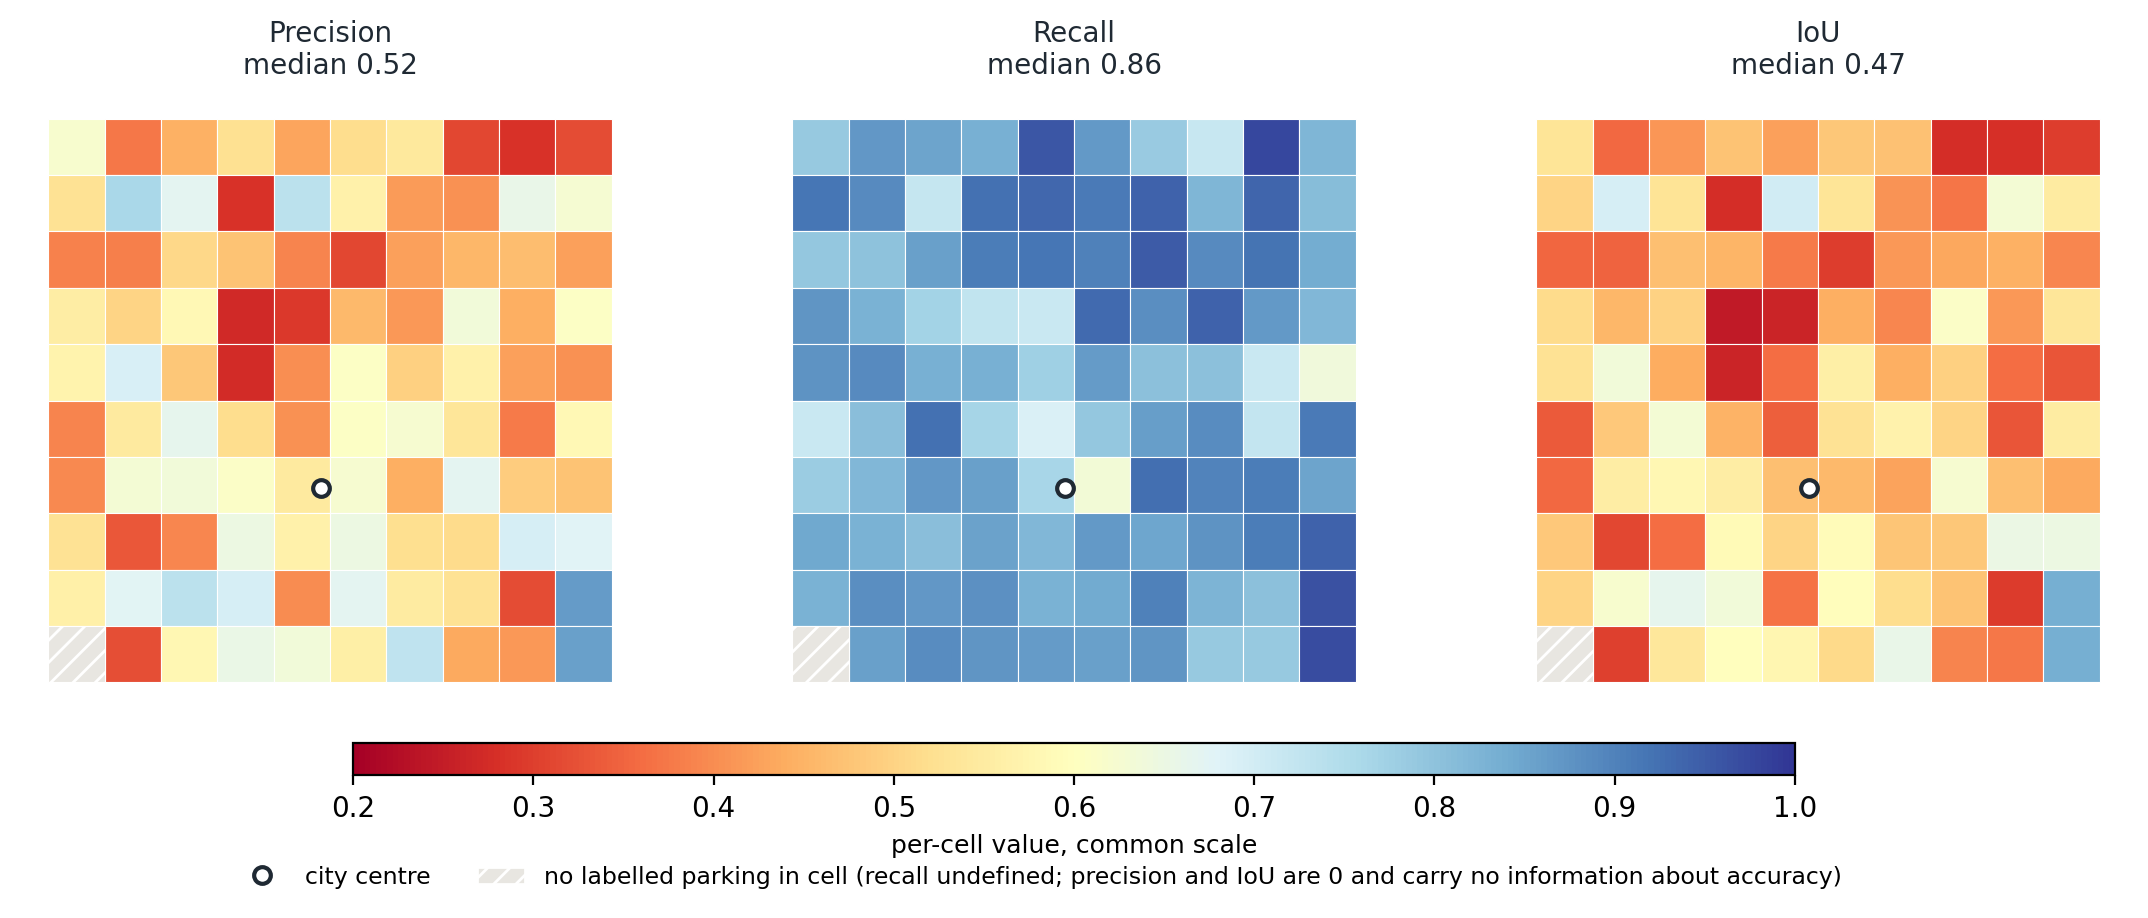
\includegraphics[width=\linewidth,height=0.82\textheight,keepaspectratio]{figures/fig_accuracy_maps.png}
\caption{Precision, recall and IoU for each 1 km² cell, on a common colour scale. Recall is generally high and less spatially variable than precision. One cell contains no labelled parking and is hatched.}
\label{fig:4.1}
\end{figure}\restoreparskip

Figure 4.1 shows that the asymmetry is not an artefact of aggregation: recall is generally high and varies less across the study area, while precision ranges from below 0.3 to above 0.8 between neighbouring cells. The macro figures fall below the micro figures on all three measures --- precision 0.514 against 0.571 --- indicating that cells contributing little parking area perform worse than the area-weighted total suggests.

Restricting the reference to the more confident labels does not improve precision; it lowers it, from 0.571 to 0.529. Since removing labels can only convert true positives into false positives, this establishes that the confidence-1 labels are not a substantial source of the measured over-prediction.

\hypertarget{false-positives}{%
\section{False positives}\label{false-positives}}

False-positive area is 2.0937 km². Figure 4.2 shows what it is made of.

\begin{figure}[htbp]
\centering
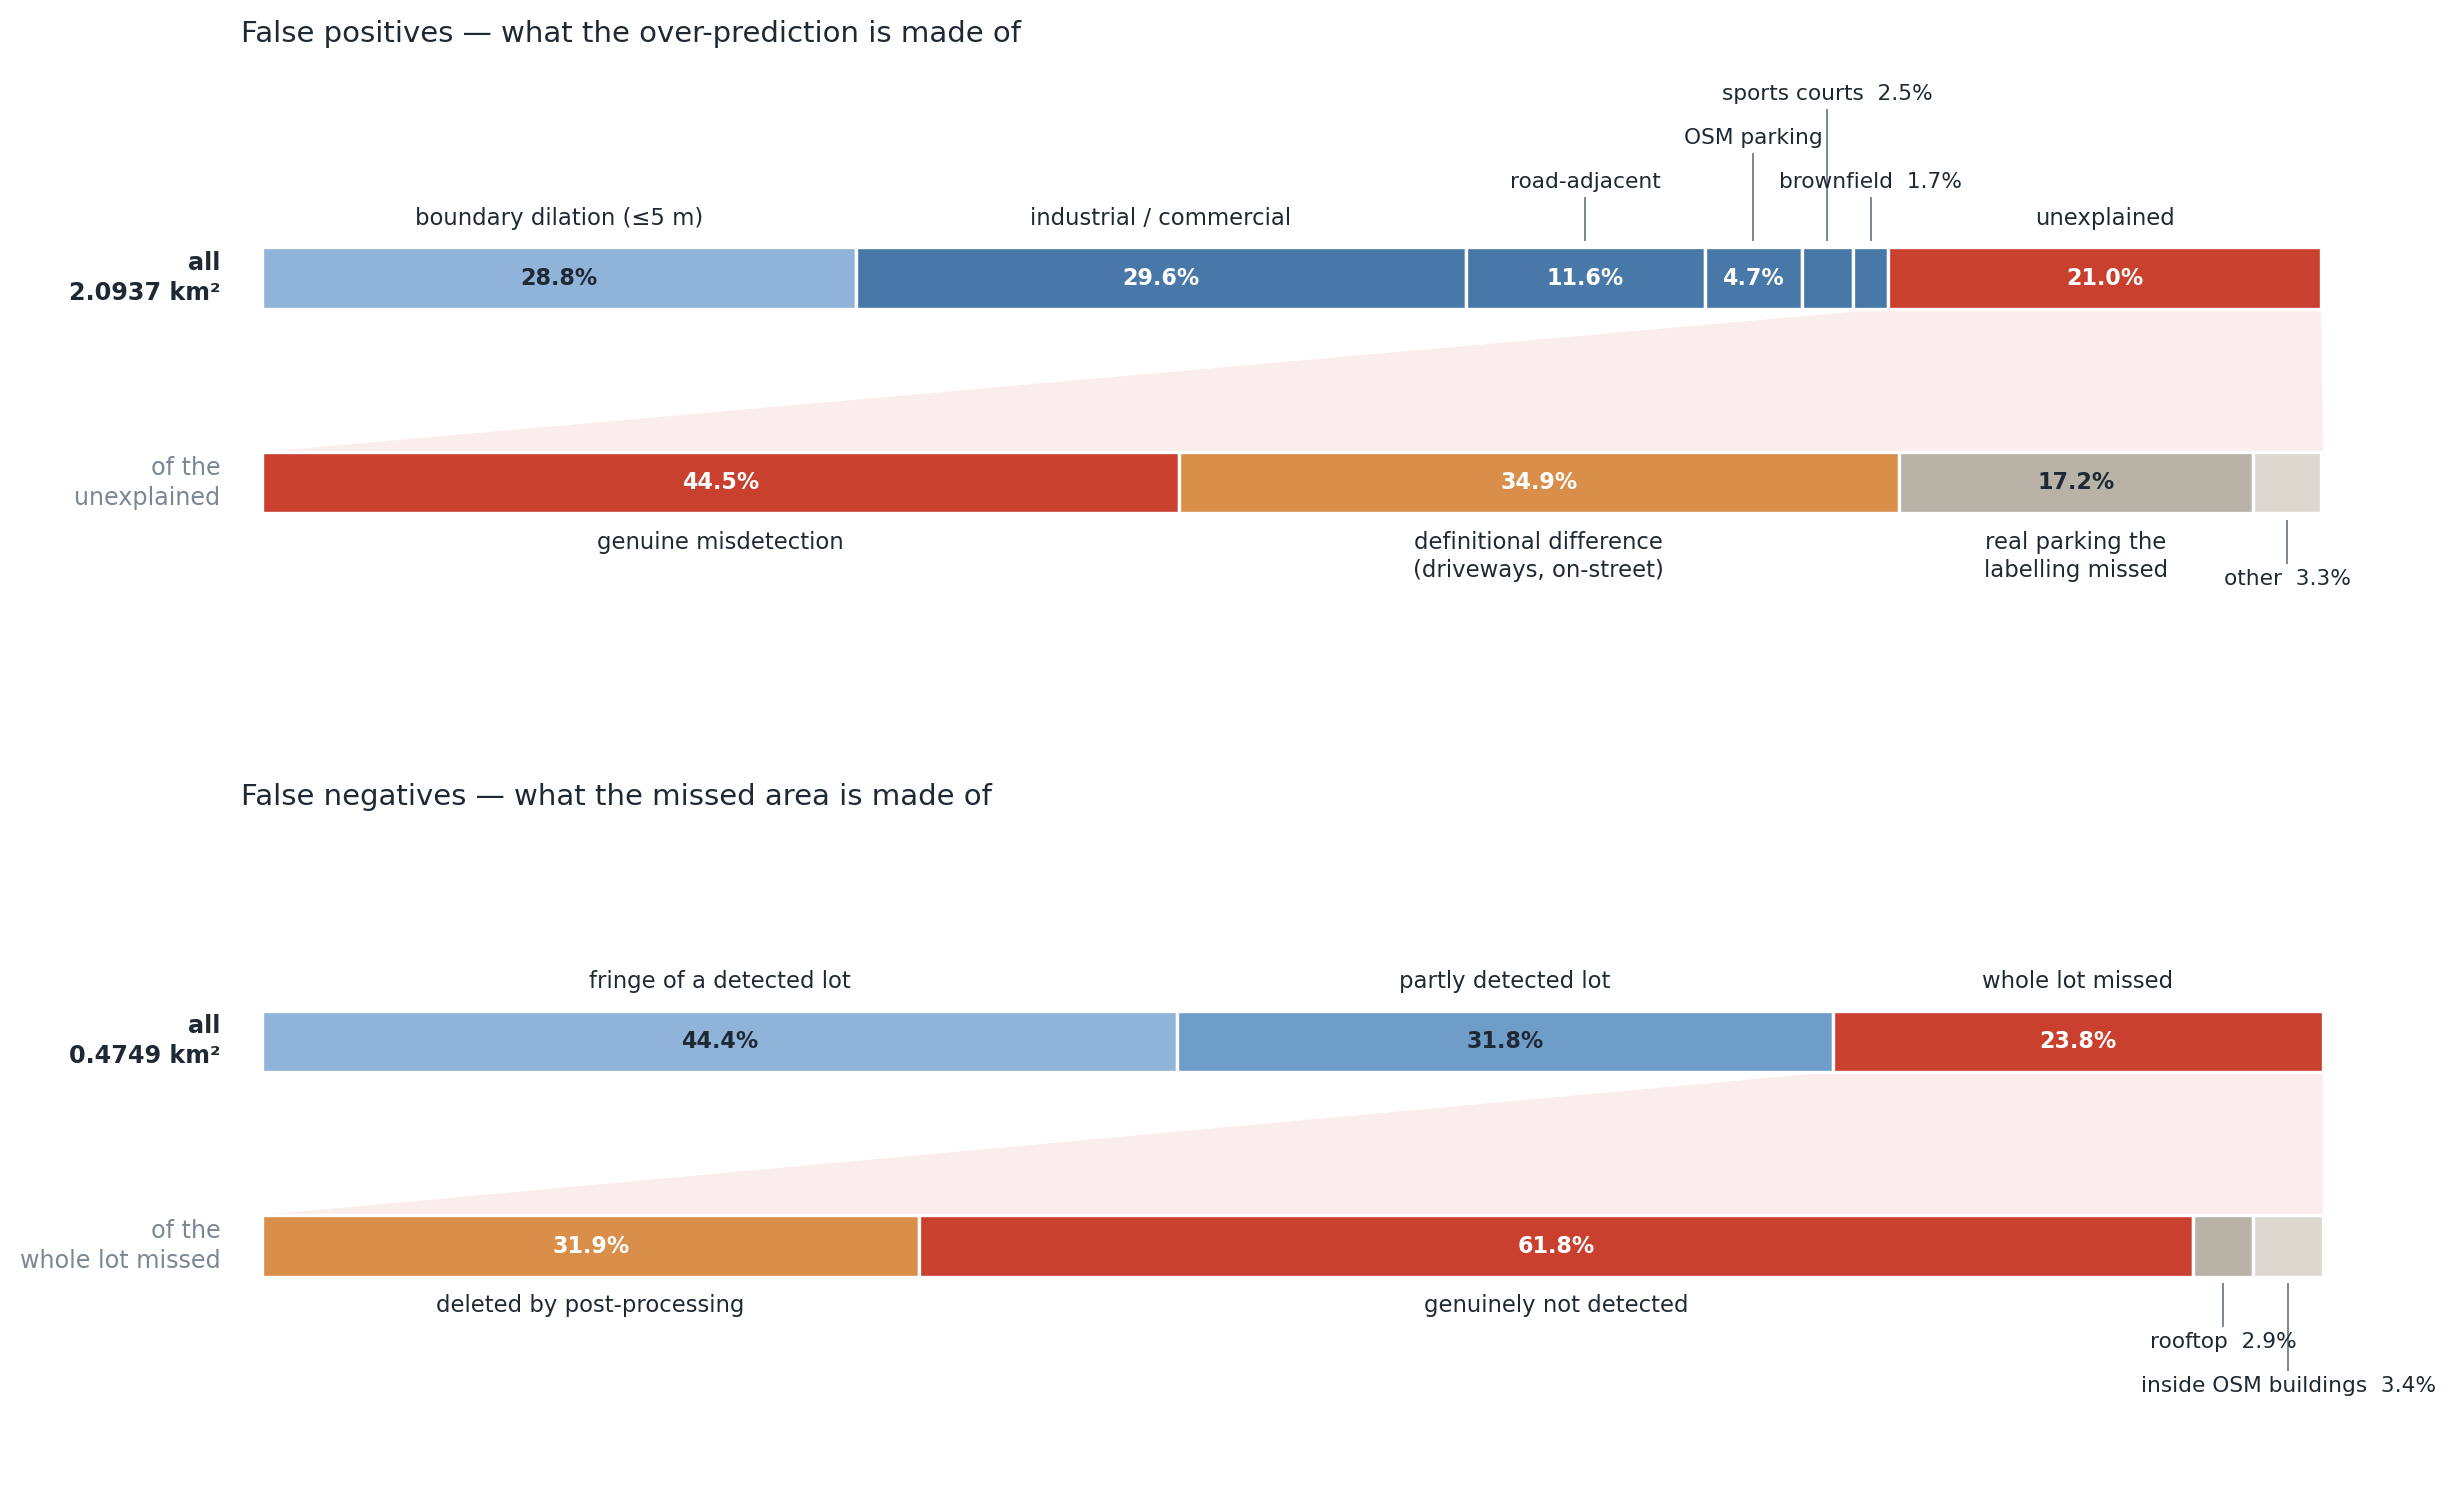
\includegraphics[width=\linewidth,height=0.82\textheight,keepaspectratio]{figures/fig_error_composition.png}
\caption{Composition of false-positive area (upper) and false-negative area (lower). In each case the lower bar expands the residual segment of the bar above it. Exclusive shares are of all FP or FN and sum to 100\%.}
\label{fig:4.2}
\end{figure}\restoreparskip

\textbf{Boundary effects account for a substantial minority.} False-positive area lying within a fixed distance of a labelled car park --- the model finding the right lot and drawing it too large --- is 17.3\% at 2 m, 28.8\% at 5 m and 36.3\% at 10 m. The three thresholds are reported because 5 m is a working convention; the value chosen shifts this component by nearly twenty percentage points.

\textbf{Attribution of the standalone remainder.} Table 4.2 gives the exclusive partition alongside the unordered diagnostic.

\begin{table}[htbp]
\centering
\caption{Where false-positive area falls. The two columns have different denominators and are not differences of one another: exclusive shares are assigned once each and sum to 100\%, while unordered overlaps are measured against all FP independently and may overlap one another.}\label{tab:4.2}
\begin{adjustbox}{max width=\textwidth}
\begin{tabular}{@{}lrr@{}}
\toprule
Layer & Exclusive (\% of all FP) & Unordered overlap (\% of all FP) \\
\midrule
Boundary dilation (≤ 5 m) & 28.8 & --- \\
Industrial / commercial land & 29.6 & \textbf{52.8} \\
Road-adjacent (+6 m) & 11.6 & 16.9 \\
OSM parking & 4.7 & 9.1 \\
Sports courts & 2.5 & 3.1 \\
Brownfield & 1.7 & 2.3 \\
Buildings & 0.0 & 0.0 \\
\textbf{Unexplained} & \textbf{21.0} & --- \\
\bottomrule
\end{tabular}
\end{adjustbox}
\end{table}
\restoreparskip

Industrial and commercial land coincides with over half of all false-positive area. Buildings account for none, because OSM building footprints have already been subtracted at the post-processing stage; false positives on buildings the OSM data does not record fall into the unexplained residual. Moving industrial land from an early position in the peeling order to last changes its exclusive share from 30.0\% to 29.6\%, so the attribution is not an artefact of the ordering.

\textbf{The unexplained residual divides into three unlike things.} Stratified sampling of 70 chips (Figure 4.3) estimates that 44.5\% of the residual is genuine misdetection --- grey hardstanding, goods yards, sports courts, unpaved ground and unmapped houses --- while 34.9\% is real parking that the annotation rules deliberately exclude, principally private driveways (20.2\%) and on-street parking (14.7\%). A further 17.2\% is parking the labelling itself missed. Percentages are of the sampling frame defined in §3.6.

\hypertarget{false-negatives}{%
\section{False negatives}\label{false-negatives}}

Missed area is 0.4749 km², 14.6\% of labelled parking. Measured against the prediction, 33.4\% of it lies within 2 m of something the model did find, 54.1\% within 5 m and 69.4\% within 10 m.

\textbf{Most missed area is the edge of a car park the model found.} Classifying missed area by how much of its parent lot the model covered gives a more useful split than any distance threshold:

\begin{table}[htbp]
\centering
\caption{Missed area by the state of the car park it belongs to.}\label{tab:4.3}
\begin{adjustbox}{max width=\textwidth}
\begin{tabular}{@{}llrrr@{}}
\toprule
Class & Coverage of the lot & Lots & Missed area (km²) & Share of FN \\
\midrule
Fringe of a well-detected lot & \textgreater{} 70\% & 1,638 & 0.2108 & 44.4\% \\
Partly detected & 10--70\% & 278 & 0.1510 & 31.8\% \\
\textbf{Whole lot missed} & ≤ 10\% & \textbf{121} & \textbf{0.1131} & \textbf{23.8\%} \\
\bottomrule
\end{tabular}
\end{adjustbox}
\end{table}
\restoreparskip

Nearly half of all missed area belongs to lots the model detected to better than 70\%. Only the third row is a detection failure in any useful sense, and it is not what it appears: 31.9\% of it was found by the model and then deleted by post-processing, with a further 2.9\% labelled as rooftop and 3.4\% falling inside OSM building footprints. After these automated attributions, 0.0699 km² remains unresolved, or 2.1\% of labelled area. The separate sampled assessment in §4.6 shows that reference--imagery disagreement also contributes to the whole-lot-miss population.

\textbf{Detection tracks size and annotator confidence.}

\begin{table}[htbp]
\centering
\caption{Detection rate by lot size and by labelling confidence.}\label{tab:4.4}
\begin{adjustbox}{max width=\textwidth}
\begin{tabular}{@{}lrrr@{}}
\toprule
Lot size & Lots & Mean detection rate & Missed entirely \\
\midrule
\textless{} 200 m² & 47 & 0.658 & \textbf{19.1\%} \\
200--500 m² & 563 & 0.763 & 8.2\% \\
500--1,000 m² & 573 & 0.805 & 5.4\% \\
1,000--2,500 m² & 559 & 0.852 & 3.0\% \\
2,500--5,000 m² & 182 & 0.850 & 4.9\% \\
\textgreater{} 5,000 m² & 113 & 0.864 & \textbf{1.8\%} \\
\bottomrule
\end{tabular}
\end{adjustbox}
\end{table}
\restoreparskip

\begin{table}[htbp]
\centering
\begin{adjustbox}{max width=\textwidth}
\begin{tabular}{@{}lrrr@{}}
\toprule
Confidence & Lots & Mean detection rate & Missed entirely \\
\midrule
1 (uncertain) & 435 & 0.713 & 10.6\% \\
2 & 1,137 & 0.829 & 3.8\% \\
3 (clear) & 465 & 0.856 & 5.4\% \\
\bottomrule
\end{tabular}
\end{adjustbox}
\end{table}
\restoreparskip

Lots below 200 m² are missed outright more than ten times as often as lots above 5,000 m². Detection is also lowest where the annotator was least certain, which indicates that part of the measured error reflects genuine ambiguity in the target rather than model deficiency.

\textbf{What the unresolved whole-lot population looks like.} Sampling of 42 chips estimates the composition of the residual as: not parking in the Digimap imagery 41.8\%, irregular layout 23.3\%, obscured by shadow or canopy 9.8\%, unusual surface 9.2\%, no cars present 6.3\%, vans and lorries rather than cars 5.2\%, and no markings 3.7\%.

\begin{figure}[htbp]
\centering
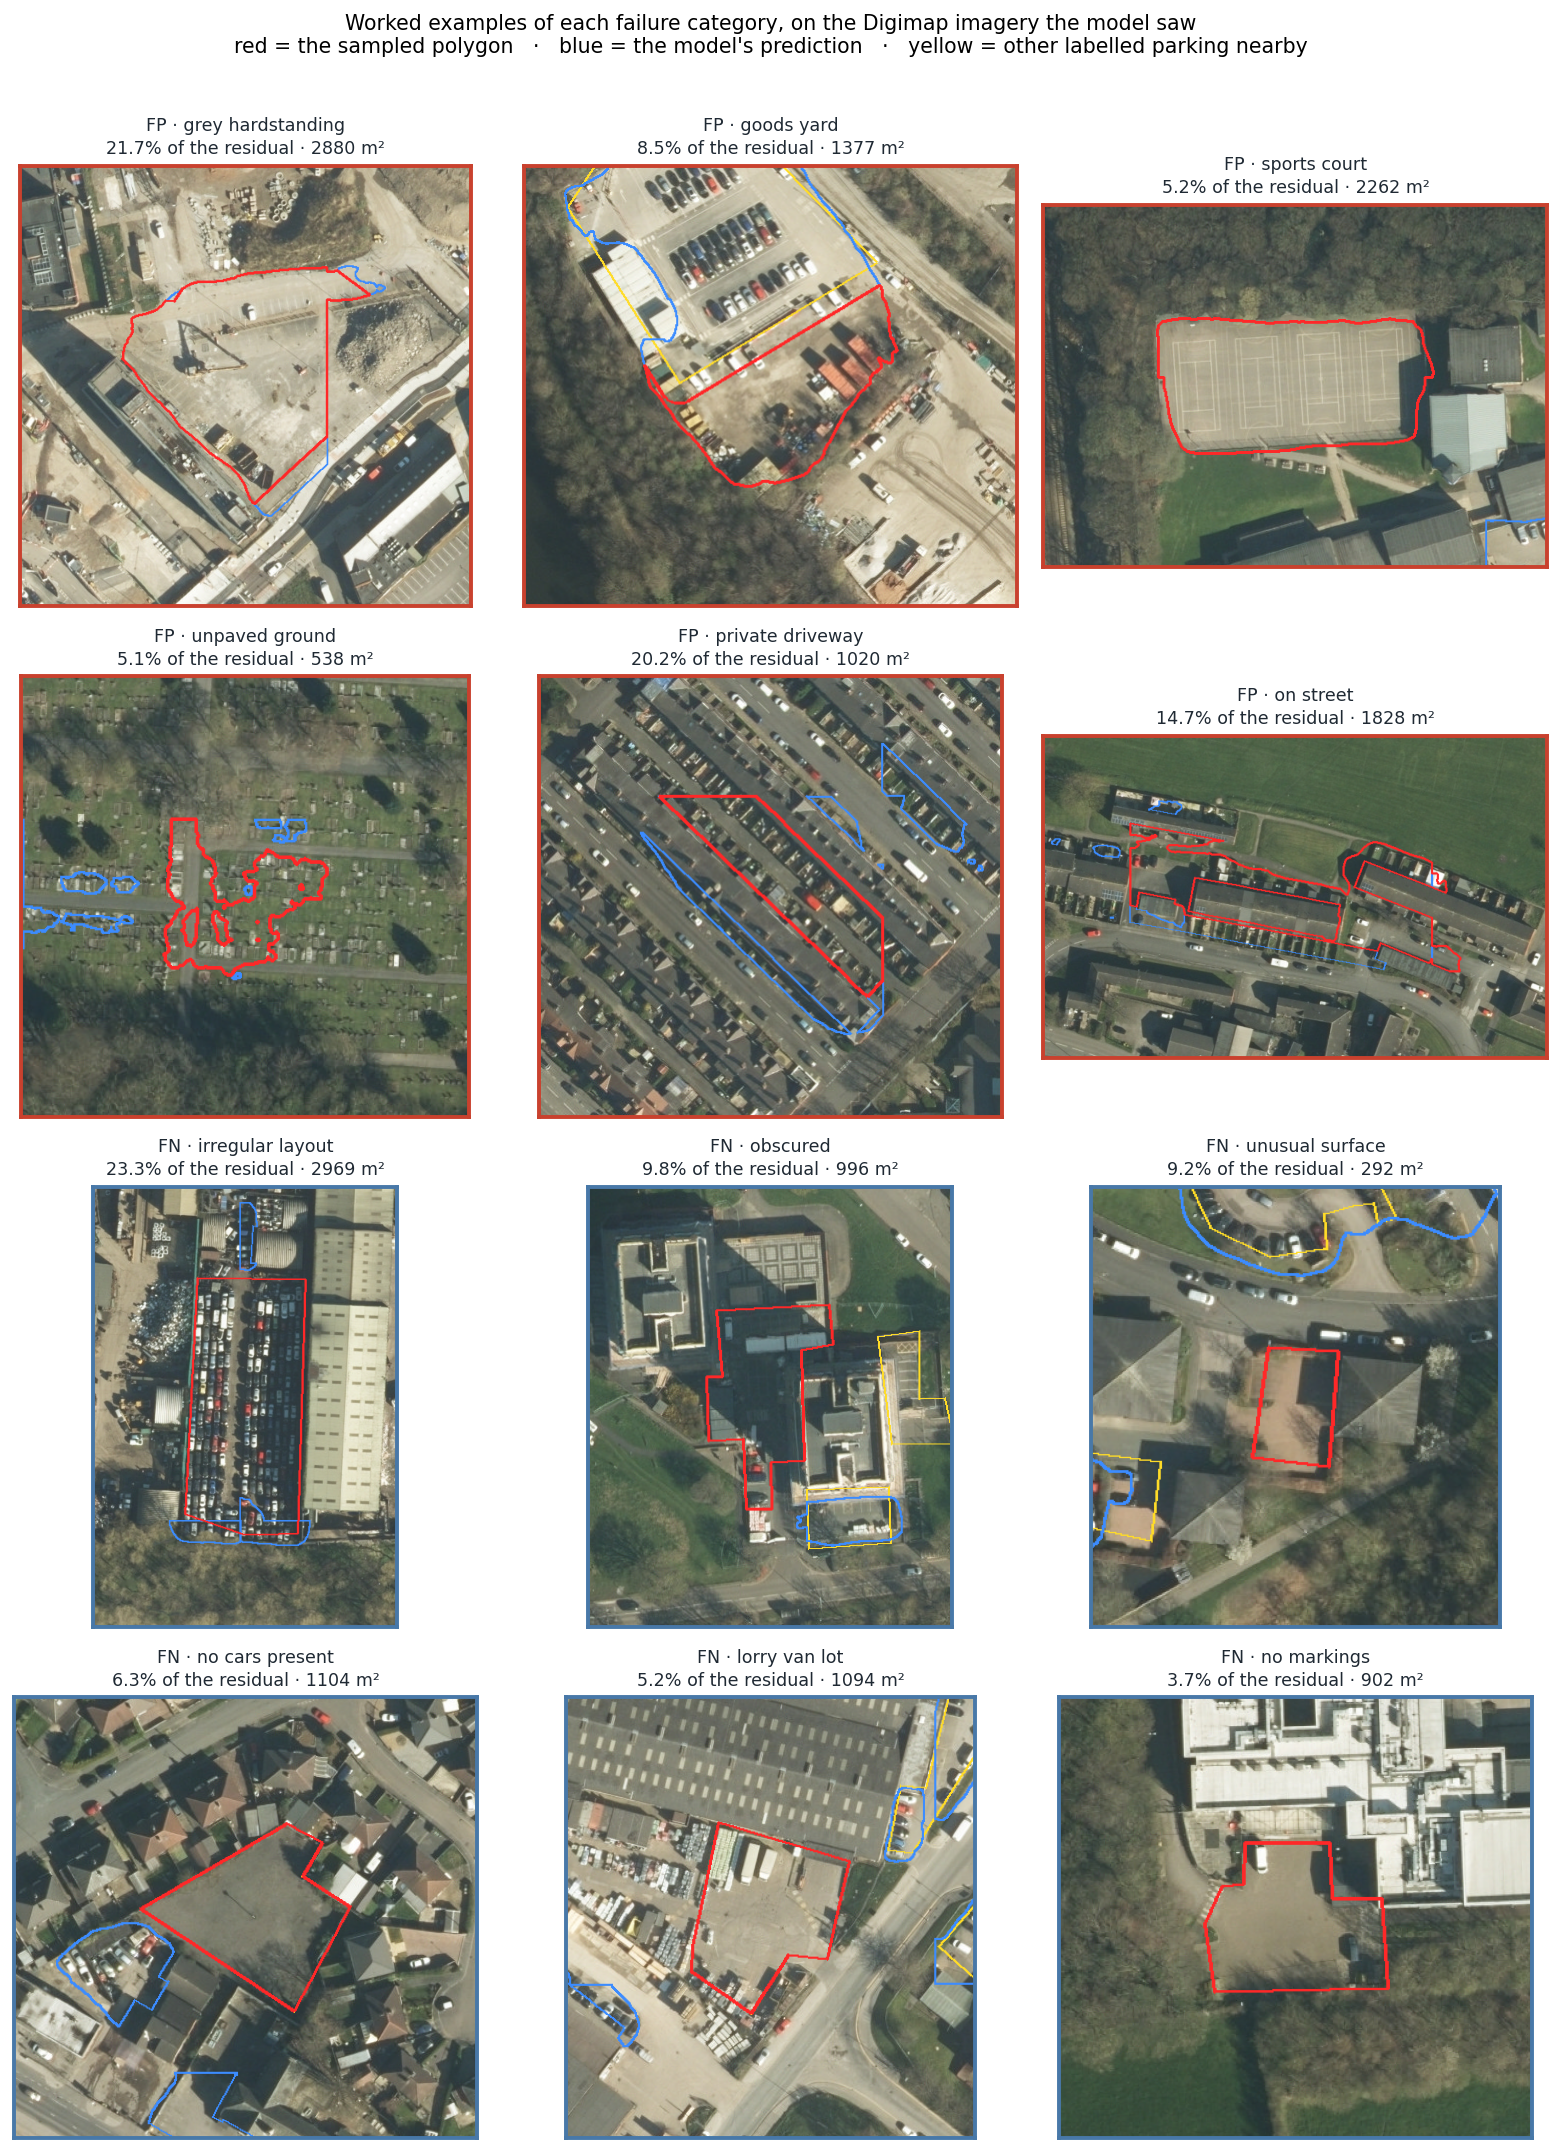
\includegraphics[width=\linewidth,height=0.82\textheight,keepaspectratio]{figures/fig_error_chips.png}
\caption{One worked example of each of twelve failure categories, on the Digimap imagery the model was given. Red outlines the sampled polygon, blue the model's prediction, yellow other labelled parking nearby.}
\label{fig:4.3}
\end{figure}\restoreparskip

Irregular layout was identified in 11 of 42 chips and absent markings in one. Although the resulting 3.7\% estimate for absent markings is imprecise, its interval remains well below that for irregular layout --- 3.7\% {[}0.6, 9.8{]} against 23.3\% {[}16.9, 31.1{]}. The evidence therefore supports the ordering, rather than a precise ratio: irregular arrangement was the most frequently identified mechanism and unmarked surfacing among the least, revising the expectation in §2.5 that unmarked surfaces would be the principal difficulty.

\hypertarget{post-processing-and-the-reference-layers-as-filters}{%
\section{Post-processing and the reference layers as filters}\label{post-processing-and-the-reference-layers-as-filters}}

\begin{figure}[htbp]
\centering
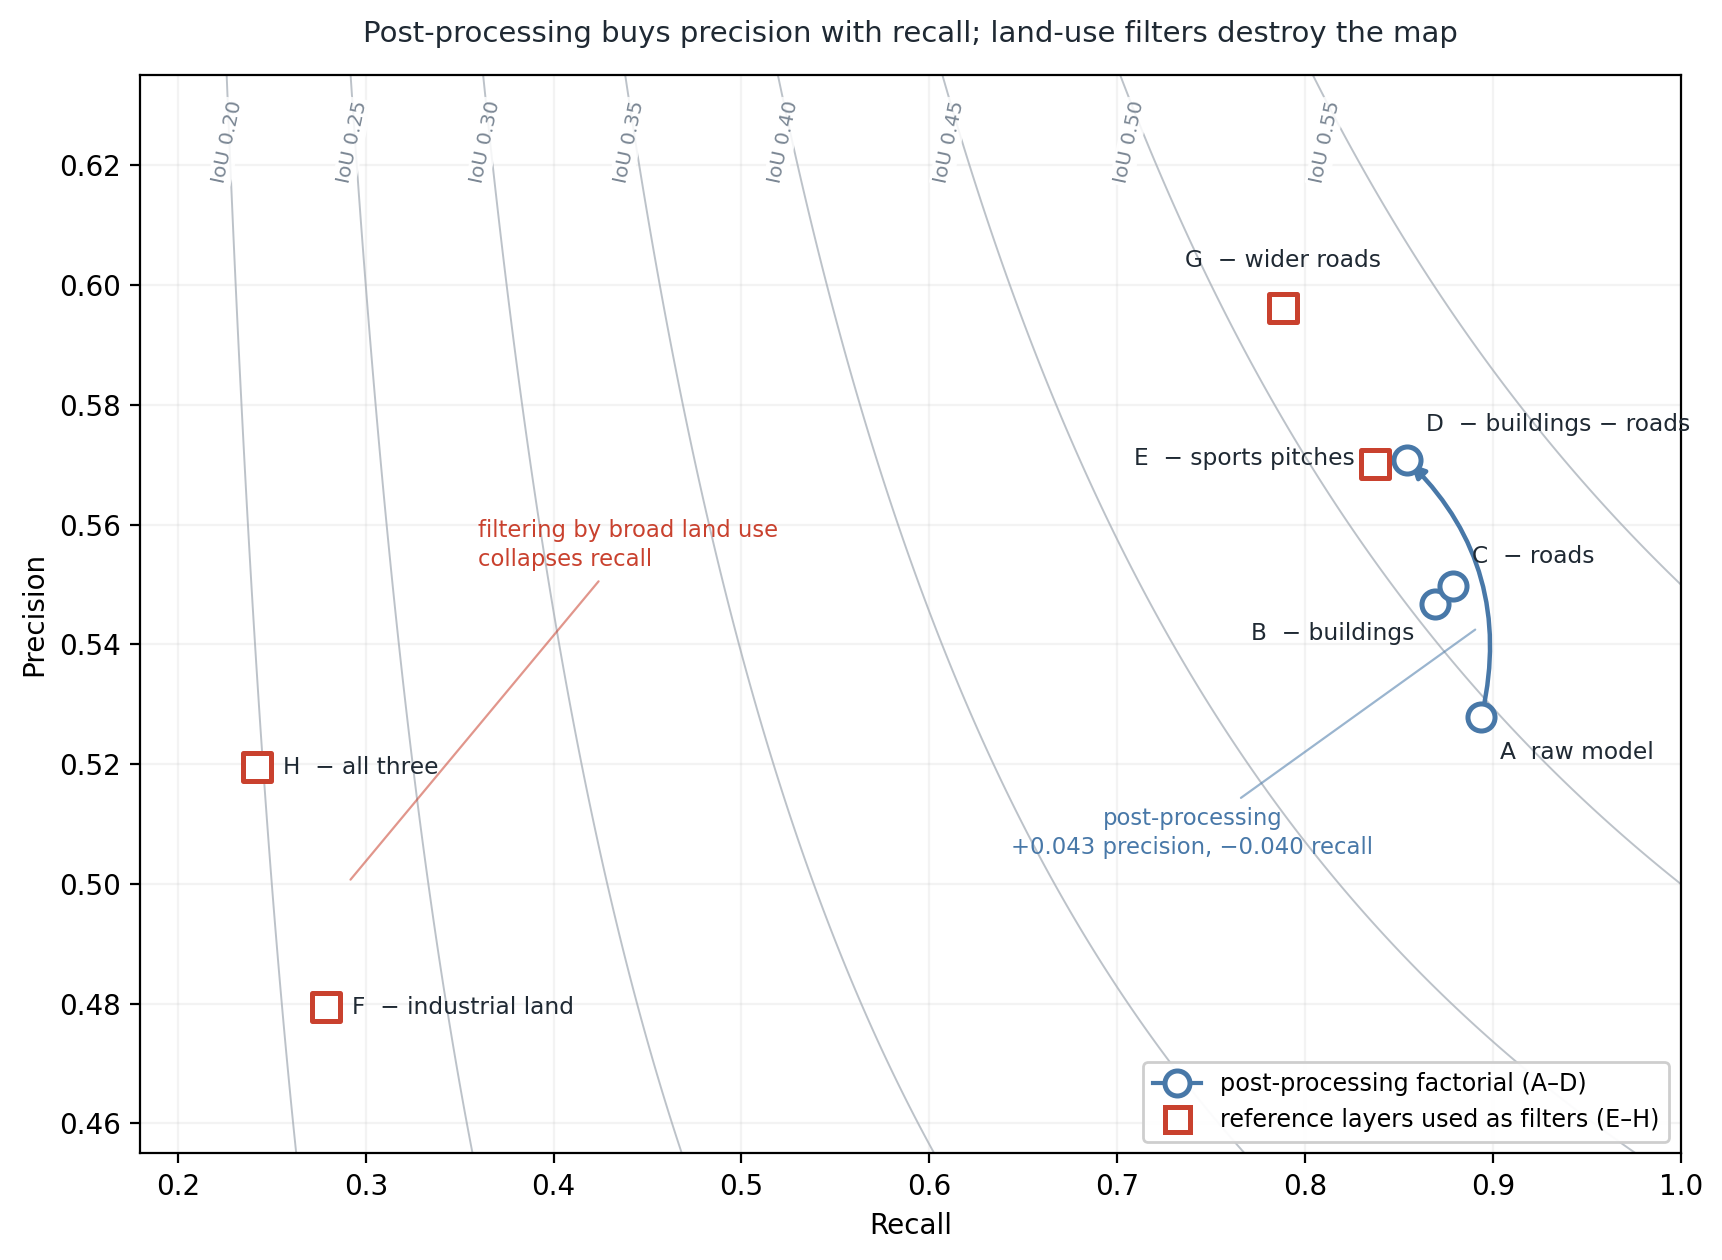
\includegraphics[width=\linewidth,height=0.82\textheight,keepaspectratio]{figures/fig_ablation.png}
\caption{The eight variants on the precision--recall plane, with IoU iso-lines. Circles are the building-and-road subtraction factorial; squares are reference layers applied as filters.}
\label{fig:4.4}
\end{figure}\restoreparskip

\begin{table}[htbp]
\centering
\caption{Ablation. Variants A--D vary the building and road subtractions; E--H apply further layers as filters to the finished map.}\label{tab:4.5}
\begin{adjustbox}{max width=\textwidth}
\begin{tabular}{@{}lrrr@{}}
\toprule
Variant & Precision & Recall & IoU \\
\midrule
A pre-subtraction output & 0.5278 & 0.8939 & 0.4967 \\
B − buildings & 0.5467 & 0.8691 & 0.5051 \\
C − roads & 0.5498 & 0.8789 & 0.5111 \\
\textbf{D − buildings − roads} & \textbf{0.5708} & \textbf{0.8543} & \textbf{0.5202} \\
E − sports pitches & 0.5701 & 0.8373 & 0.5132 \\
\textbf{F − industrial land} & 0.4794 & \textbf{0.2789} & \textbf{0.2140} \\
G − wider roads & \textbf{0.5962} & 0.7884 & 0.5140 \\
H − all three & 0.5195 & 0.2419 & 0.1976 \\
\bottomrule
\end{tabular}
\end{adjustbox}
\end{table}
\restoreparskip

Reconstructing D from the pre-subtraction output in a single operation reproduces the pipeline's own tile-by-tile result to within 0.0\% on all three measures, so the ablation isolates the two subtractions.

The two subtractions together raise precision by 0.043 and lower recall by 0.040, for a net IoU gain of 0.024. Each contributes roughly half. Applied as filters, the further layers behave quite differently. Subtracting industrial and commercial land --- the layer that coincided with 52.8\% of false-positive area --- collapses recall from 0.854 to 0.279 and IoU from 0.520 to 0.214, because supermarket and retail-park car parks sit on exactly that land. Widening the road buffers is the only variant to raise precision (to 0.596), and it still lowers IoU.

\textbf{The pipeline creates a blind spot of its own.} Sixteen labelled lots, 0.0395 km² or 1.21\% of the reference, are rooftop parking.

\begin{table}[htbp]
\centering
\caption{Rooftop parking, before and after post-processing.}\label{tab:4.6}
\begin{adjustbox}{max width=\textwidth}
\begin{tabular}{@{}lr@{}}
\toprule
Measure & Value \\
\midrule
Recall on rooftop lots, before subtraction & \textbf{0.916} \\
Recall on rooftop lots, after subtraction & \textbf{0.115} \\
Recall on non-rooftop lots, before subtraction & 0.894 \\
Rooftop area falling inside OSM buildings & 85.6\% \\
Rooftop area detected then removed & \textbf{80.1\%} \\
\bottomrule
\end{tabular}
\end{adjustbox}
\end{table}
\restoreparskip

The pre-subtraction output detects rooftop parking slightly \emph{better} than ground-level parking. Subtracting building footprints removes four fifths of it.

\hypertarget{accuracy-and-location}{%
\section{Accuracy and location}\label{accuracy-and-location}}

\begin{table}[htbp]
\centering
\caption{Correlations with per-cell precision, recall and IoU (Pearson r, p in brackets). Recall statistics use the 99 cells with labelled parking.}\label{tab:4.7}
\begin{adjustbox}{max width=\textwidth}
\begin{tabular}{@{}lrrrr@{}}
\toprule
Metric & Distance & Parking share & Distance \textbar{} parking share & Parking share \textbar{} distance \\
\midrule
\textbf{Precision} & −0.172 (0.087) & \textbf{+0.536 (\textless0.0001)} & +0.186 (0.065) & \textbf{+0.540 (\textless0.0001)} \\
Recall & +0.181 (0.073) & +0.103 (0.313) & +0.289 (0.004) & +0.250 (0.013) \\
IoU & −0.127 (0.208) & \textbf{+0.515 (\textless0.0001)} & +0.229 (0.022) & \textbf{+0.540 (\textless0.0001)} \\
\bottomrule
\end{tabular}
\end{adjustbox}
\end{table}
\restoreparskip

Distance from the city centre does not predict precision. The share of a cell given over to parking does, strongly, and continues to do so after controlling for distance. The reverse does not hold: controlling for parking share, the distance effect is not significant. Distance and parking share are themselves correlated at −0.562.

All three metrics are reported to avoid selective presentation, but only precision is interpreted here. The partial correlations for recall and IoU reach significance while their raw correlations do not, and their signs reverse between the two; with n = 100 and two strongly correlated predictors this pattern is not a stable basis for a claim.

Read across distance bands, precision falls from 0.584 within 1 km to 0.485 beyond 4 km while recall stays between 0.70 and 0.86 (see Figure 4.5 and Appendix B). The band means move with parking share, not with distance.

\begin{figure}[htbp]
\centering
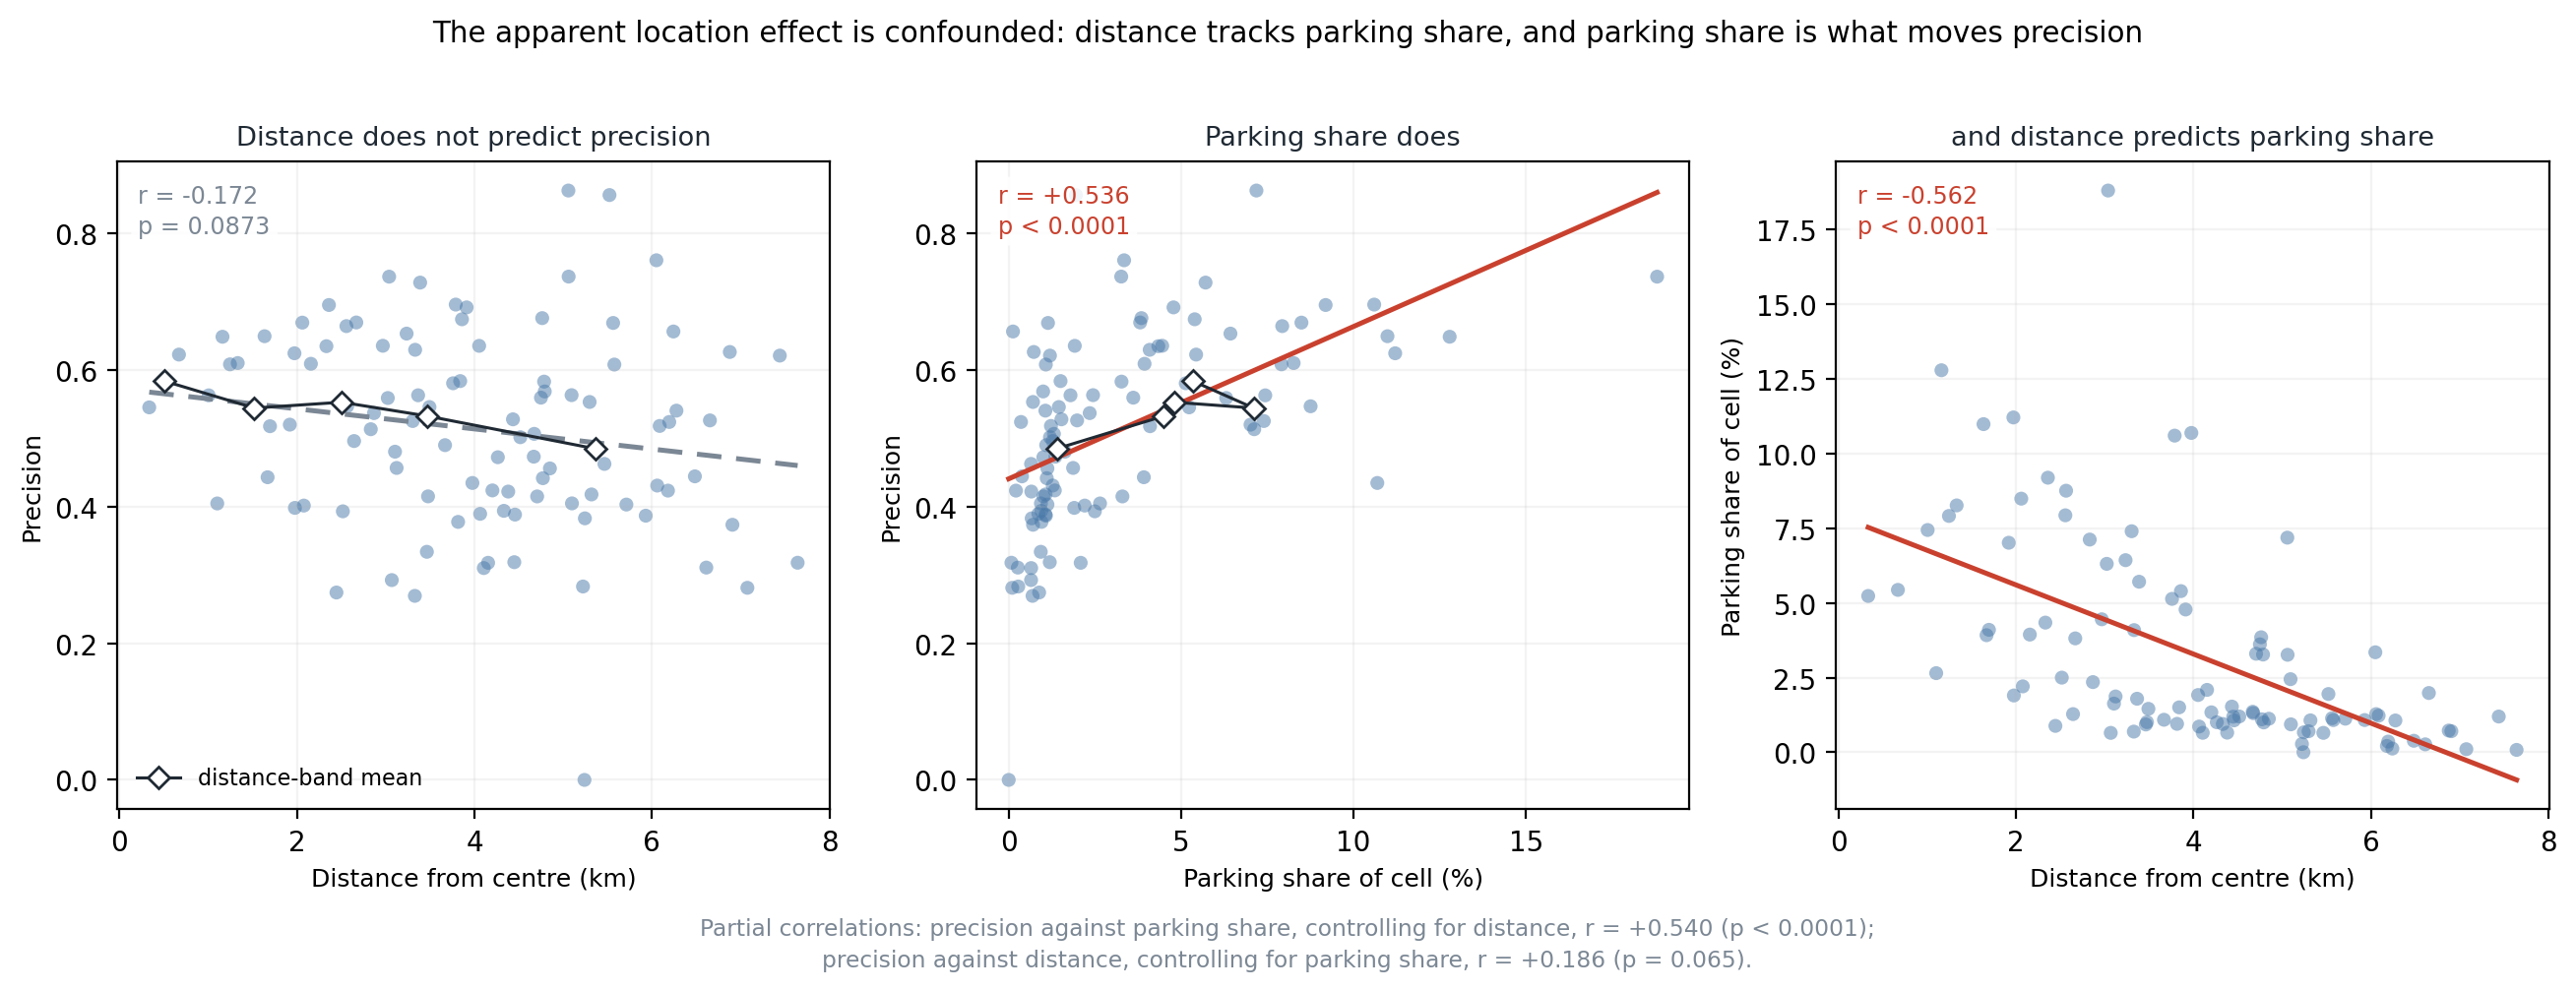
\includegraphics[width=\linewidth,height=0.82\textheight,keepaspectratio]{figures/fig_accuracy_vs_location.png}
\caption{Per-cell precision against distance and against parking share, and parking share against distance. Solid red fits are significant at p \textless{} 0.05; the dashed grey fit is not. Diamonds are distance-band means.}
\label{fig:4.5}
\end{figure}\restoreparskip

\hypertarget{sampled-corrections-and-what-the-reference-is-worth}{%
\section{Sampled corrections, and what the reference is worth}\label{sampled-corrections-and-what-the-reference-is-worth}}

Applying the sampled estimates as corrections gives four cumulative variants:

\begin{table}[htbp]
\centering
\caption{Accuracy under cumulative correction.}\label{tab:4.8}
\begin{adjustbox}{max width=\textwidth}
\begin{tabular}{@{}lrrrrr@{}}
\toprule
Variant & Reference (km²) & Prediction (km²) & Precision & Recall & IoU \\
\midrule
\textbf{1 As measured} & 3.2597 & 4.8785 & \textbf{0.5708} & \textbf{0.8543} & \textbf{0.5202} \\
2 + reference-side (−0.0313, not parking in the imagery) & 3.2284 & 4.8785 & 0.5708 & 0.8626 & 0.5233 \\
3 + prediction-side (+0.0667, parking the labelling missed) & 3.2951 & 4.8785 & 0.5845 & 0.8654 & 0.5358 \\
\textbf{4 Effective (−0.1358, definitional exclusions removed)} & 3.2951 & 4.7427 & \textbf{0.6012} & 0.8654 & \textbf{0.5498} \\
\bottomrule
\end{tabular}
\end{adjustbox}
\end{table}
\restoreparskip

Across the four variants, precision rises from 0.571 to 0.601, about half of the gain coming from the final removal of on-street parking and private driveways --- real parking excluded by the target definition rather than model error. Recall changes only from 0.854 to 0.865. For variant 4, the stratified bootstrap gives 95\% intervals of {[}0.5941, 0.6090{]} for precision, {[}0.8635, 0.8675{]} for recall and {[}0.5434, 0.5569{]} for IoU; its precision interval remains above the measured 0.5708. The headline pattern is therefore unchanged, and variant 1 remains the primary result.

\textbf{OpenStreetMap, assessed against the same reference.} OSM records 1.7641 km² of parking across 985 polygons, against 3.2597 km² across 2,037 labelled polygons. It overlaps only 1.1882 km², or 36.5\% of labelled parking, leaving 63.5\% absent from OSM. Similar median polygon areas (763 and 799 m²) suggest that this incompleteness is not explained simply by polygon size. Within the 0.2610 km² sampling frame of OSM parking polygons above 100 m² and no more than 10\% covered by the labels, 63.2\% is estimated to show no parking in the model-input imagery. The 11 sampled features in that category had a median last-edit year of 2025, so stale OSM records are not supported as a general explanation, subject to the timestamp limitation in §3.8.

\hypertarget{the-extent-and-distribution-of-surface-parking}{%
\section{The extent and distribution of surface parking}\label{the-extent-and-distribution-of-surface-parking}}

\begin{table}[htbp]
\centering
\caption{Surface parking as a share of land, by distance band.}\label{tab:4.9}
\begin{adjustbox}{max width=\textwidth}
\begin{tabular}{@{}lrrrr@{}}
\toprule
Band & Cells & Labelled & Model & Calibrated (km²) \\
\midrule
\textless{} 1 km & 2 & 5.33\% & 6.42\% & 0.086 \\
\textbf{1--2 km} & 11 & \textbf{7.11\%} & 10.35\% & 0.761 \\
2--3 km & 14 & 4.80\% & 7.19\% & 0.673 \\
3--4 km & 22 & 4.50\% & 6.53\% & 0.959 \\
\textgreater{} 4 km & 51 & 1.39\% & 2.29\% & 0.781 \\
\textbf{Whole area} & 100 & \textbf{3.26\%} & 4.88\% & 3.2595 \\
\bottomrule
\end{tabular}
\end{adjustbox}
\end{table}
\restoreparskip

The calibrated column applies the whole-area factor from §3.9. Its whole-area value is an identity; the band rows show residuals when that citywide factor is applied within each band (−19.6\% to +10.0\%), not an independent transfer test.

The complete-coverage reference contains 3.2597 km² of surface parking, or 3.26\% of the 100 km² study area. The sampled reference corrections in §4.6 raise this to 3.2951 km² (3.30\%), a shift of less than 0.1 percentage points.

Parking share peaks at 7.11\% in the 1--2 km band and then falls monotonically to 1.39\% beyond 4 km. The apparent central dip to 5.33\% is uncertain because the \textless1 km band contains only two cells. Across cells, the distribution is strongly right-skewed: mean 3.26\%, median 1.71\%, maximum 18.81\%, with six cells above 10\%.

\begin{figure}[htbp]
\centering

\includegraphics[width=\linewidth,height=0.82\textheight,keepaspectratio]{figures/parking_extent.png}
\caption{Labelled parking share by cell (white circle: City Square), labelled and predicted shares against distance, and the distribution of labelled shares across the 100 cells.}
\label{fig:4.6}
\end{figure}\restoreparskip

\textbf{Calibration and the grain at which it holds.} For a map with precision \emph{p} and recall \emph{r}, reference-equivalent area is estimated as predicted area × \emph{p}/\emph{r} (§3.9); here, 4.8785 × \emph{p}/\emph{r} = 3.2595 km². This is an identity on the cells used to fit the factor. Table 4.10 tests it on held-out cells.

\begin{table}[htbp]
\centering
\caption{Error of the calibrated estimate on cells excluded from fitting the factor.}\label{tab:4.10}
\begin{adjustbox}{max width=\textwidth}
\begin{tabular}{@{}llrrrr@{}}
\toprule
Scheme & Held out & Tests & Mean error & 5th--95th pct. & Within ±25\% \\
\midrule
\textbf{Random half split} & 50 cells & 200 & +0.3\% & \textbf{−6.6\% to +7.8\%} & 100\% \\
Leave one distance band out & 1 band & 5 & −2.9\% & −16.9\% to +10.6\% & --- \\
\textbf{Leave one cell out} & 1 cell & 99 & +16.5\% & −22.0\% to +80.5\% & \textbf{63\%} \\
\bottomrule
\end{tabular}
\end{adjustbox}
\end{table}
\restoreparskip

Across the 200 random half splits, the central 90\% of held-out errors runs from −6.6\% to +7.8\%, showing that a factor fitted on half the city transfers to a comparable sub-area within the same city. This is not an uncertainty interval for the directly labelled 3.26\%. At 1 km², the estimator becomes unstable: only 63\% of cells fall within ±25\%, and the +16.5\% mean is inflated by small denominators (median absolute error 0.0035 km² against mean labelled area 0.0329 km²).

\begin{figure}[htbp]
\centering

\includegraphics[width=\linewidth,height=0.82\textheight,keepaspectratio]{figures/calibration_transfer.png}
\caption{Held-out calibration errors under the three schemes. Red lines mark medians and dashed black lines means; the distance-band panel contains only five tests.}
\label{fig:4.7}
\end{figure}\restoreparskip

\chapter{Discussion}\input{chapters/05_discussion}
\chapter{Conclusion}This dissertation tested whether a US-trained surface-parking segmentation model can be used to measure off-street surface parking in a British city. The model was applied to 100 km² of Leeds exactly as released, with no UK training data in the primary analysis, and evaluated against 2,037 manually labelled car parks drawn to the source model's own target definition. The error was then decomposed rather than merely reported: attributed exhaustively against independent reference layers, characterised by stratified sampling of 142 image chips adjudicated on the imagery the model actually consumed, and tested by ablation of the building- and road-subtraction stage.

The transfer works asymmetrically. Recall of 0.854 is generally high and less spatially variable than precision, which is 0.571; the model predicts 1.50 times the labelled parking area. Accuracy within the city tracks not distance from the centre but how much parking a cell contains --- an apparent location effect that dissolves once parking abundance is controlled for.

Recognition failure is not the dominant explanation: automated attribution leaves 0.0699 km² of whole-lot FN unresolved, 2.1\% of labelled area and under 3\% of all error area, while sampled adjudication separately identifies reference--imagery disagreement. Boundary placement is the largest single component, at 28.8\% of false-positive and 54.1\% of false-negative area, with the remainder split between confusions with particular look-alike surfaces, disagreement over what counts as parking, and pipeline artefacts. Among the sampled unresolved whole-lot population, irregular arrangement was the most frequently identified mechanism and absent markings among the least. Building and road subtraction is a real trade, buying 0.043 of precision for 0.040 of recall, but it also creates a blind spot of its own: the pre-subtraction output detects rooftop parking better than ground-level parking, and building subtraction deletes four fifths of it.

Under that measured reliability, surface parking covers 3.26\% of the study area as labelled, or 3.30\% after the sampled corrections. The highest shares fall in the inner 2 km, reaching 7.11\% in the 1--2 km band, with a clear decline beyond; and it is strongly concentrated: a median cell gives over 1.71\%, while six exceed 10\%.

\textbf{Contributions.} Four, in ascending order of transferability beyond this case. First, an empirical measurement of how a published US-trained parking segmentation model behaves in a British city, previously unavailable. Second, a reusable method for decomposing area-based segmentation error into boundary effects, attributable confusions, definitional disagreement and pipeline artefacts --- a decomposition that turns a single accuracy figure into a statement about which uses survive. Third, evidence that a correction step justified by a sound premise can create a systematic blind spot, which is an argument for evaluating correction stages rather than assuming them. Fourth, a hold-out test of the spatial grain at which a standard area-calibration factor remains reliable: it holds to about ±7\% at half-city scale within Leeds and fails at the scale of a single square kilometre.

\textbf{Future work.} The calibration factor reduces to a ratio of labelled to predicted area, so testing whether it transfers between cities requires labelled totals over a sample of cells rather than a repeat of the full error analysis undertaken here. This makes a multi-city test more tractable, although its cost and between-city validity remain untested. The typology points to a direction for training data: irregularly arranged car parks rather than simply unmarked ones, on the strength of eleven sampled chips. Imagery carrying a near-infrared band would test the one expected failure this study could not examine. A supplementary experiment (Appendix C) narrows what that validation should compare. Generic fine-tuning improved raw-pixel IoU while trading recall for precision; weighting the loss by positional error categories added neither overall nor selective gain, and its operating points were matched or bettered by adjusting the generic model's threshold alone. The next question
is whether, and which kind of, local supervision earns its labelling cost --- a comparison of zero-shot use, area calibration, generic fine-tuning and visually targeted fine-tuning, judged on locating parking, estimating area, and the precision--recall trade-off each implies.

The Leeds results show that a transferred model cannot be trusted to measure parking area without local validation. Within the same city, local calibration supports area estimation at half-city scale; whether that finding transfers between cities remains open.


% =====================================================================
%  References
% =====================================================================
\chapter*{References}
\addcontentsline{toc}{chapter}{References}
\markboth{References}{References}
\begin{hangparas}{1.5em}{1}
Bates, J. and Leibling, D. (2012) \emph{Spaced out: perspectives on parking policy}. London: RAC Foundation.

Berry, T., Dronen, N., Jackson, B. and Endres, I. (2019) `Parking lot instance segmentation from satellite imagery through associative embeddings', in \emph{Proceedings of the 27th ACM SIGSPATIAL International Conference on Advances in Geographic Information Systems}. New York: Association for Computing Machinery, pp.~528--531. \url{doi:10.1145/3347146.3359364}.

Cheng, B., Girshick, R., Dollár, P., Berg, A.C. and Kirillov, A. (2021) `Boundary IoU: improving object-centric image segmentation evaluation', in \emph{Proceedings of the IEEE/CVF Conference on Computer Vision and Pattern Recognition}. Available at: \url{https://openaccess.thecvf.com/content/CVPR2021/papers/Cheng_Boundary_IoU_Improving_Object-Centric_Image_Segmentation_Evaluation_CVPR_2021_paper.pdf} (Accessed: 13 August 2026).

Cochran, W.G. (1977) \emph{Sampling techniques}. 3rd edn. New York: John Wiley \& Sons.

Csurka, G., Larlus, D. and Perronnin, F. (2013) `What is a good evaluation measure for semantic segmentation?', in \emph{Proceedings of the British Machine Vision Conference 2013}. Durham: BMVA Press. Available at: \url{https://www.bmva-archive.org.uk/bmvc/2013/Papers/paper0032/paper0032.pdf} (Accessed: 13 August 2026).

Devillers, R., Bédard, Y., Jeansoulin, R. and Moulin, B. (2007) `Towards spatial data quality information analysis tools for experts assessing the fitness for use of spatial data', \emph{International Journal of Geographical Information Science}, 21(3), pp.~261--282. \url{doi:10.1080/13658810600911879}.

Foody, G.M. (2002) `Status of land cover classification accuracy assessment', \emph{Remote Sensing of Environment}, 80(1), pp.~185--201. \url{doi:10.1016/S0034-4257(01)00295-4}.

Foody, G.M. (2005) `Local characterization of thematic classification accuracy through spatially constrained confusion matrices', \emph{International Journal of Remote Sensing}, 26(6), pp.~1217--1228. \url{doi:10.1080/01431160512331326521}.

Goodchild, M.F. (2007) `Citizens as sensors: the world of volunteered geography', \emph{GeoJournal}, 69(4), pp.~211--221. \url{doi:10.1007/s10708-007-9111-y}.

Habermehl, V. and McFarlane, C. (2025) `The density dialectic: between hard and gentle densification in London', \emph{International Journal of Urban and Regional Research}, 49(3), pp.~569--586. \url{doi:10.1111/1468-2427.13319}.

Haklay, M. (2010) `How good is volunteered geographical information? A comparative study of OpenStreetMap and Ordnance Survey datasets', \emph{Environment and Planning B: Planning and Design}, 37(4), pp.~682--703. \url{doi:10.1068/b35097}.

Hoehne, C.G., Chester, M.V., Fraser, A.M. and King, D.A. (2019) `Valley of the sun-drenched parking space: the growth, extent, and implications of parking infrastructure in Phoenix', \emph{Cities}, 89, pp.~186--198. \url{doi:10.1016/j.cities.2019.02.007}.

Hong, D. et al.~(2023) `Cross-city matters: a multimodal remote sensing benchmark dataset for cross-city semantic segmentation using high-resolution domain adaptation networks', \emph{Remote Sensing of Environment}, 299, 113856. \url{doi:10.1016/j.rse.2023.113856}.

Hurst-Tarrab, N., Chang, L., Gonzalez-Mendoza, M. and Hernandez-Gress, N. (2020) `Robust parking block segmentation from a surveillance camera perspective', \emph{Applied Sciences}, 10(15), 5364. \url{doi:10.3390/app10155364}.

Jiao, L. (2015) `Urban land density function: a new method to characterize urban expansion', \emph{Landscape and Urban Planning}, 139, pp.~26--39. \url{doi:10.1016/j.landurbplan.2015.02.017}.

Lange, M., Kovacevic, L. and Johnson, Z. (2026) \emph{Course correction: how to densify British cities}. London: Centre for Cities.

Livingstone, N., Fiorentino, S. and Short, M. (2021) `Planning for residential ``value''? London's densification policies and impacts', \emph{Buildings and Cities}, 2(1), pp.~203--219. \url{doi:10.5334/bc.88}.

Lv, J., Shen, Q., Lv, M., Li, Y., Shi, L. and Zhang, P. (2023) `Deep learning-based semantic segmentation of remote sensing images: a review', \emph{Frontiers in Ecology and Evolution}, 11, 1201125. \url{doi:10.3389/fevo.2023.1201125}.

Lyu, S. et al.~(2025) \emph{Deep learning based domain adaptation methods in remote sensing: a comprehensive survey}. arXiv:2510.15615. Available at: \url{https://arxiv.org/abs/2510.15615} (Accessed: 12 August 2026).

Maggiori, E., Tarabalka, Y., Charpiat, G. and Alliez, P. (2017) `Can semantic labeling methods generalize to any city? The Inria aerial image labeling benchmark', in \emph{2017 IEEE International Geoscience and Remote Sensing Symposium (IGARSS)}. Fort Worth, TX: IEEE, pp.~3226--3229. \url{doi:10.1109/IGARSS.2017.8127684}.

Ministry of Housing, Communities and Local Government (MHCLG) (2024) \emph{National Planning Policy Framework}. London: MHCLG.

Olofsson, P., Foody, G.M., Herold, M., Stehman, S.V., Woodcock, C.E. and Wulder, M.A.~(2014) `Good practices for estimating area and assessing accuracy of land change', \emph{Remote Sensing of Environment}, 148, pp.~42--57. \url{doi:10.1016/j.rse.2014.02.015}.

Openshaw, S. (1984) \emph{The modifiable areal unit problem}. Concepts and Techniques in Modern Geography 38. Norwich: Geo Books.

Qiam, S., Devunuri, S. and Lehe, L.J. (2025) `A pipeline and NIR-enhanced dataset for parking lot segmentation', in \emph{2025 IEEE/CVF Winter Conference on Applications of Computer Vision (WACV)}. IEEE, pp.~1227--1236.

Roberts, D.R. et al.~(2017) `Cross-validation strategies for data with temporal, spatial, hierarchical, or phylogenetic structure', \emph{Ecography}, 40(8), pp.~913--929. \url{doi:10.1111/ecog.02881}.

Scharnhorst, E. (2018) \emph{Quantified parking: comprehensive parking inventories for five U.S. cities}. Washington, DC: Research Institute for Housing America.

Sehra, S.S., Singh, J. and Rai, H.S. (2013) `Assessment of OpenStreetMap data --- a review', \emph{International Journal of Computer Applications}, 76(16), pp.~17--20.

Shoup, D.C. (2005) \emph{The high cost of free parking}. Chicago: Planners Press, American Planning Association.

Stehman, S.V. and Foody, G.M. (2019) `Key issues in rigorous accuracy assessment of land cover products', \emph{Remote Sensing of Environment}, 231, 111199. \url{doi:10.1016/j.rse.2019.05.018}.

Stehman, S.V. and Wickham, J.D. (2011) `Pixels, blocks of pixels, and polygons: choosing a spatial unit for thematic accuracy assessment', \emph{Remote Sensing of Environment}, 115(12), pp.~3044--3055. \url{doi:10.1016/j.rse.2011.06.007}.

Xie, E., Wang, W., Yu, Z., Anandkumar, A., Alvarez, J.M. and Luo, P. (2021) `SegFormer: simple and efficient design for semantic segmentation with transformers', \emph{Advances in Neural Information Processing Systems}, 34, pp.~12077--12090.

Yin, Y., Hu, W., Tran, A., Kruppa, H., Zimmermann, R. and Ng, S.-K. (2022) `A context-enriched satellite imagery dataset and an approach for parking lot detection', in \emph{2022 IEEE/CVF Winter Conference on Applications of Computer Vision (WACV)}. IEEE, pp.~1371--1380. \url{doi:10.1109/WACV51458.2022.00146}.

Zhou, Q., Wang, S. and Liu, Y. (2022) `Exploring the accuracy and completeness patterns of global land-cover/land-use data in OpenStreetMap', \emph{Applied Geography}, 145, 102742. \url{doi:10.1016/j.apgeog.2022.102742}.

\end{hangparas}

% =====================================================================
%  Appendices
% =====================================================================
\appendix
\addtocontents{toc}{\protect\vspace{0.6em}}

\chapter{Manual annotation protocol}These are the rules under which the 2,037 reference car parks of §3.2 were labelled. They are reproduced in full because the measured precision depends on where the scope line was drawn as much as on what the model can see (§5.5), so the protocol has to be inspectable rather than summarised.

\hypertarget{basis}{%
\section{Basis}\label{basis}}

The rules follow the annotation method of the US-trained model applied here (Qiam, Devunuri and Lehe, 2025). The same rules are used so that the accuracy figures are valid: ground-truth labels must follow the definition the model was trained on. Labelling was carried out in QGIS over the Google Satellite basemap.

\hypertarget{target}{%
\section{Target}\label{target}}

Off-street surface parking: open-air parking surfaces visible from above, outside public roads. Labels are binary (parking / non-parking). The use served is not recorded, as it cannot be judged reliably from imagery. No minimum-size threshold is applied --- all off-street surface parking is labelled regardless of size, to match the definition the model was trained on.

\hypertarget{identifying-parking}{%
\section{Identifying parking}\label{identifying-parking}}

An area is labelled as parking where it has marked parking bays, or --- where markings are absent --- parked cars and a layout of bays and aisles that clearly show parking use. Areas whose use is unclear are left unlabelled or marked confidence 1.

\textbf{Include}

\begin{itemize}
\tightlist
\item
  Surface car parks, whatever use they serve.
\item
  Parking bays and the internal aisles that connect them.
\item
  Rooftop parking where the parking surface is visible from above.
\end{itemize}

\textbf{Exclude}

\begin{itemize}
\tightlist
\item
  On-street parking.
\item
  Multi-storey or underground car parks with no visible parking surface.
\end{itemize}

\textbf{Treated as non-parking}, and also the common look-alikes the model most often confuses:

\begin{itemize}
\tightlist
\item
  Sports courts, storage or depot yards, and other non-parking hardstanding.
\item
  Buildings, roads, pavements and landscaping.
\end{itemize}

\hypertarget{driveways}{%
\section{Driveways}\label{driveways}}

Only very short entrances belonging to a car park are included. Longer access roads are excluded, so that the labels do not teach the model to recognise roads (Qiam, Devunuri and Lehe, 2025).

\textbf{Supplementary rule --- residential parking.} Individual single-house driveways or forecourts --- a few cars, clearly one household --- are not labelled: they are private curtilage, not a car park. Shared or communal residential parking courts serving several dwellings are labelled. This extends the source authors' driveway rule rather than contradicting it: a single-house driveway is private access, like the driveways they exclude, whereas a communal court is genuine off-street surface parking under their target. This is the one point at which the protocol narrows the source definition, and the resulting difference is held separate in the error analysis of §4.2 rather than counted as model error.

\hypertarget{boundary}{%
\section{Boundary}\label{boundary}}

\begin{itemize}
\tightlist
\item
  Draw along the edge of the paving, not the parcel boundary.
\item
  Keep one car park as one polygon, even where it is split by planting islands.
\item
  Align to the current image. Where OpenStreetMap or another reference is out of date --- a demolished building, for instance --- follow the current image. OpenStreetMap parking is used only as a starting reference, never as ground truth.
\end{itemize}

\hypertarget{attributes}{%
\section{Attributes}\label{attributes}}

\begin{table}[htbp]
\centering
\begin{adjustbox}{max width=\textwidth}
\begin{tabular}{@{}ll@{}}
\toprule
Field & Description \\
\midrule
\texttt{confidence} & 3 = clear, 2 = fairly clear, 1 = uncertain \\
\texttt{notes} & Optional note for ambiguous cases \\
\bottomrule
\end{tabular}
\end{adjustbox}
\end{table}
\restoreparskip

The main validation uses the full label set. Results for the confidence 2--3 subset are reported alongside it in Appendix B as a sensitivity analysis, so that the effect of the uncertain labels is visible rather than assumed.

\hypertarget{why-these-rules-and-how-reliable-they-are}{%
\section{Why these rules, and how reliable they are}\label{why-these-rules-and-how-reliable-they-are}}

The model is validated against these labels, so the labels must match the definition the model was trained on. The rules therefore follow Qiam, Devunuri and Lehe (2025) as closely as possible: the same off-street surface target, pavement-edge boundaries, rooftop parking only where the deck is visible, and no minimum-size cut-off.

Annotating surface parking as a binary polygon class is an established approach in comparable aerial-imagery datasets --- APKLOT (Hurst-Tarrab et al., 2020) and Grab-Pklot (Yin et al., 2022) are both built this way --- so the approach is not ad hoc. APKLOT likewise fixes its target with an explicit include-and-exclude list, though it segments parking blocks rather than whole car parks, so the internal aisles labelled here fall outside its target; Grab-Pklot annotates whole carparks, the closer analogue to the target used here. The data were labelled by a single annotator, and no second labelling pass or inter-annotator agreement coefficient was produced; §5.5 treats this as a limitation, and Table 4.4 reports how far detection differs for the lots the annotator marked uncertain. Any point at which these rules differ from the source protocol is noted above, and error caused by such definitional difference is separated from model error in §4.2.

\hypertarget{sources}{%
\section{Sources}\label{sources}}

\begin{itemize}
\tightlist
\item
  Qiam, S., Devunuri, S. and Lehe, L.J. (2025) `A pipeline and NIR-enhanced dataset for parking lot segmentation', \emph{WACV}.
\item
  Hurst-Tarrab, N., Chang, L., Gonzalez-Mendoza, M. and Hernandez-Gress, N. (2020) `Robust parking block segmentation from a surveillance camera perspective', \emph{Applied Sciences}, 10(15), 5364.
\item
  Yin, Y., Hu, W., Tran, A., Kruppa, H., Zimmermann, R. and Ng, S.-K. (2022) `A context-enriched satellite imagery dataset and an approach for parking lot detection', \emph{WACV}, pp.~1371--1380.
\end{itemize}

\chapter{Per-cell validation and accuracy by distance}Supporting tables for §4.1 and §4.5. The study area is a 10 × 10 grid of 1 km² cells; every cell is validated against the manual reference of Appendix A. \texttt{all} uses the complete label set, \texttt{c23} the confidence 2--3 subset, so that the effect of the confidence filter is visible throughout.

\hypertarget{overall-validation}{%
\section{Overall validation}\label{overall-validation}}

\begin{table}[htbp]
\centering
\begin{adjustbox}{max width=\textwidth}
\begin{tabular}{@{}lrrrrrr@{}}
\toprule
Aggregation & Manual km² & Model km² & Model ÷ manual & Precision & Recall & IoU \\
\midrule
Area-weighted, all labels & 3.2597 & 4.8785 & 1.497 & 0.5708 & 0.8543 & 0.5202 \\
Area-weighted, confidence 2--3 & 2.9790 & 4.8785 & 1.638 & 0.5287 & 0.8658 & 0.4886 \\
Mean of cells, all labels & --- & --- & --- & 0.5136 & 0.8468 & 0.4697 \\
Mean of cells, confidence 2--3 & --- & --- & --- & 0.4756 & 0.8617 & 0.4408 \\
\bottomrule
\end{tabular}
\end{adjustbox}
\end{table}
\restoreparskip

\hypertarget{accuracy-by-distance-band}{%
\section{Accuracy by distance band}\label{accuracy-by-distance-band}}

\begin{table}[htbp]
\centering
\begin{adjustbox}{max width=\textwidth}
\begin{tabular}{@{}lrrrrrrrr@{}}
\toprule
Band (km) & Cells & Mean dist. km & Manual km² & Model km² & Mean parking share & Mean precision & Mean recall & Mean IoU \\
\midrule
\textless1 & 2 & 0.503 & 0.107 & 0.128 & 0.053 & 0.584 & 0.698 & 0.462 \\
1-2 & 11 & 1.52 & 0.782 & 1.139 & 0.071 & 0.545 & 0.828 & 0.489 \\
2-3 & 14 & 2.504 & 0.672 & 1.007 & 0.048 & 0.553 & 0.86 & 0.509 \\
3-4 & 22 & 3.471 & 0.989 & 1.436 & 0.045 & 0.533 & 0.837 & 0.485 \\
\textgreater4 & 51 & 5.36 & 0.71 & 1.169 & 0.014 & 0.485 & 0.858 & 0.449 \\
\bottomrule
\end{tabular}
\end{adjustbox}
\end{table}
\restoreparskip

\hypertarget{correlations-with-distance-and-parking-share}{%
\section{Correlations with distance and parking share}\label{correlations-with-distance-and-parking-share}}

Partial correlations control for the other predictor. \texttt{n\ =\ 99} for recall because one cell holds no reference parking and yields no recall value.

\begin{table}[htbp]
\centering
\begin{adjustbox}{max width=\textwidth}
\begin{tabular}{@{}lrrrrr@{}}
\toprule
Test & n & Pearson r & p & Spearman ρ & p \\
\midrule
distance vs prec\_\allowbreak{}all & 100 & -0.172 & 0.0873 & -0.186 & 0.0637 \\
parking\_\allowbreak{}share vs prec\_\allowbreak{}all & 100 & 0.536 & 0.0 & 0.653 & 0.0 \\
distance vs prec\_\allowbreak{}all \textbar{} controlling parking\_\allowbreak{}share & 100 & 0.186 & 0.0646 & --- & --- \\
parking\_\allowbreak{}share vs prec\_\allowbreak{}all \textbar{} controlling distance & 100 & 0.54 & 0.0 & --- & --- \\
distance vs rec\_\allowbreak{}all & 99 & 0.181 & 0.073 & 0.161 & 0.1124 \\
parking\_\allowbreak{}share vs rec\_\allowbreak{}all & 99 & 0.103 & 0.3125 & 0.084 & 0.4097 \\
distance vs rec\_\allowbreak{}all \textbar{} controlling parking\_\allowbreak{}share & 99 & 0.289 & 0.0037 & --- & --- \\
parking\_\allowbreak{}share vs rec\_\allowbreak{}all \textbar{} controlling distance & 99 & 0.25 & 0.0127 & --- & --- \\
distance vs iou\_\allowbreak{}all & 100 & -0.127 & 0.2081 & -0.16 & 0.1114 \\
parking\_\allowbreak{}share vs iou\_\allowbreak{}all & 100 & 0.515 & 0.0 & 0.639 & 0.0 \\
distance vs iou\_\allowbreak{}all \textbar{} controlling parking\_\allowbreak{}share & 100 & 0.229 & 0.0222 & --- & --- \\
parking\_\allowbreak{}share vs iou\_\allowbreak{}all \textbar{} controlling distance & 100 & 0.54 & 0.0 & --- & --- \\
distance vs parking\_\allowbreak{}share & 100 & -0.562 & 0.0 & -0.66 & 0.0 \\
\bottomrule
\end{tabular}
\end{adjustbox}
\end{table}
\restoreparskip

\hypertarget{per-cell-results}{%
\section{Per-cell results}\label{per-cell-results}}

All 100 cells, ordered by grid column then row. Cell identifiers follow the \texttt{c\textless{}col\textgreater{}r\textless{}row\textgreater{}} convention used in the project repository.

\par\addvspace{\medskipamount}\noindent
\begin{landscape}
\begingroup\scriptsize
\begin{longtable}[]{@{}lrrrrrrrrrrr@{}}
\toprule
Cell & Dist. km & Parking share & Model m² & Manual m² (all) & P & R & IoU & Manual m² (c23) & P & R & IoU \\
\midrule
\endhead
c0r0 & 7.44 & 0.0120 & 15166.2 & 11958.1 & 0.6213 & 0.788 & 0.5323 & 11438.8 & 0.6 & 0.7956 & 0.5199 \\
c0r1 & 6.65 & 0.0198 & 34517.6 & 19834.2 & 0.5264 & 0.9161 & 0.5022 & 14774.3 & 0.3933 & 0.9188 & 0.3801 \\
c0r2 & 5.93 & 0.0108 & 22064.7 & 10779.8 & 0.3869 & 0.7919 & 0.3512 & 10475.2 & 0.3731 & 0.7859 & 0.3387 \\
c0r3 & 5.30 & 0.0070 & 11121.2 & 7037.9 & 0.5534 & 0.8745 & 0.5127 & 6170.0 & 0.4827 & 0.8701 & 0.4502 \\
c0r4 & 4.79 & 0.0100 & 15406.5 & 9984.8 & 0.5688 & 0.8777 & 0.527 & 9589.1 & 0.5546 & 0.891 & 0.5193 \\
c0r5 & 4.46 & 0.0107 & 19572.6 & 10670.7 & 0.3885 & 0.7126 & 0.3359 & 10670.7 & 0.3885 & 0.7126 & 0.3359 \\
c0r6 & 4.33 & 0.0095 & 18793.0 & 9459.0 & 0.394 & 0.7827 & 0.3551 & 9459.0 & 0.394 & 0.7827 & 0.3551 \\
c0r7 & 4.43 & 0.0153 & 24464.7 & 15285.8 & 0.528 & 0.8451 & 0.4815 & 15285.8 & 0.528 & 0.8451 & 0.4815 \\
c0r8 & 4.75 & 0.0361 & 53584.5 & 36125.2 & 0.5597 & 0.8302 & 0.5022 & 33897.9 & 0.5209 & 0.8234 & 0.4686 \\
c0r9 & 5.24 & 0.0000 & 140.3 & 0.0 & 0.0 & & 0.0 & 0.0 & 0.0 & & 0.0 \\
c1r0 & 6.91 & 0.0071 & 16400.9 & 7052.4 & 0.3736 & 0.8689 & 0.3537 & 7052.4 & 0.3736 & 0.8689 & 0.3537 \\
c1r1 & 6.05 & 0.0335 & 39166.7 & 33469.1 & 0.7609 & 0.8904 & 0.6957 & 33105.2 & 0.7528 & 0.8907 & 0.6892 \\
c1r2 & 5.24 & 0.0067 & 13932.1 & 6665.4 & 0.383 & 0.8005 & 0.3496 & 6665.4 & 0.383 & 0.8005 & 0.3496 \\
c1r3 & 4.52 & 0.0120 & 19818.0 & 11971.5 & 0.5018 & 0.8307 & 0.4552 & 11971.5 & 0.5018 & 0.8307 & 0.4552 \\
c1r4 & 3.91 & 0.0478 & 61374.4 & 47794.3 & 0.6919 & 0.8885 & 0.6366 & 47667.6 & 0.6916 & 0.8904 & 0.6373 \\
c1r5 & 3.49 & 0.0145 & 21524.3 & 14536.1 & 0.546 & 0.8085 & 0.4835 & 13687.5 & 0.5079 & 0.7986 & 0.4502 \\
c1r6 & 3.33 & 0.0409 & 53347.6 & 40889.4 & 0.6298 & 0.8217 & 0.5541 & 34852.4 & 0.5428 & 0.8309 & 0.4888 \\
c1r7 & 3.46 & 0.0093 & 23073.3 & 9296.1 & 0.334 & 0.8289 & 0.3124 & 8714.3 & 0.3109 & 0.8231 & 0.2914 \\
c1r8 & 3.86 & 0.0539 & 70603.4 & 53947.6 & 0.6745 & 0.8827 & 0.619 & 49100.9 & 0.6361 & 0.9146 & 0.6004 \\
c1r9 & 4.45 & 0.0119 & 32059.6 & 11906.2 & 0.3188 & 0.8583 & 0.3028 & 9304.0 & 0.2773 & 0.9555 & 0.2738 \\
c2r0 & 6.48 & 0.0038 & 7350.5 & 3841.8 & 0.4445 & 0.8505 & 0.4123 & 2803.6 & 0.3573 & 0.9367 & 0.3489 \\
c2r1 & 5.56 & 0.0114 & 12243.9 & 11395.4 & 0.6691 & 0.7189 & 0.5304 & 11229.4 & 0.6613 & 0.721 & 0.5266 \\
c2r2 & 4.67 & 0.0131 & 22189.7 & 13104.5 & 0.5067 & 0.8579 & 0.4675 & 10796.4 & 0.4089 & 0.8404 & 0.3794 \\
c2r3 & 3.84 & 0.0150 & 19851.0 & 15031.1 & 0.584 & 0.7713 & 0.4978 & 12666.1 & 0.4883 & 0.7653 & 0.4247 \\
c2r4 & 3.11 & 0.0163 & 28269.3 & 16284.5 & 0.4806 & 0.8342 & 0.4387 & 14123.0 & 0.4397 & 0.8802 & 0.4149 \\
c2r5 & 2.56 & 0.0793 & 110231.0 & 79329.8 & 0.6645 & 0.9233 & 0.6297 & 71617.8 & 0.6047 & 0.9308 & 0.5787 \\
c2r6 & 2.33 & 0.0434 & 59548.0 & 43401.3 & 0.6351 & 0.8714 & 0.5807 & 38202.4 & 0.5722 & 0.8919 & 0.535 \\
c2r7 & 2.52 & 0.0250 & 51368.4 & 24978.6 & 0.3933 & 0.8088 & 0.3599 & 20950.9 & 0.3296 & 0.8082 & 0.3057 \\
c2r8 & 3.04 & 0.1881 & 221784.2 & 188065.4 & 0.7369 & 0.869 & 0.6633 & 181524.9 & 0.7184 & 0.8778 & 0.6531 \\
c2r9 & 3.76 & 0.0513 & 78303.1 & 51349.6 & 0.5808 & 0.8857 & 0.5403 & 41951.5 & 0.4872 & 0.9094 & 0.4647 \\
c3r0 & 6.20 & 0.0036 & 5654.1 & 3561.5 & 0.5241 & 0.8321 & 0.474 & 3561.5 & 0.5241 & 0.8321 & 0.474 \\
c3r1 & 5.22 & 0.0028 & 8997.8 & 2761.4 & 0.2832 & 0.9229 & 0.2767 & 2270.4 & 0.2444 & 0.9687 & 0.2425 \\
c3r2 & 4.26 & 0.0100 & 19307.0 & 10044.1 & 0.4725 & 0.9083 & 0.451 & 7148.7 & 0.3574 & 0.9652 & 0.3529 \\
c3r3 & 3.33 & 0.0069 & 18655.1 & 6909.9 & 0.2695 & 0.7277 & 0.2449 & 5584.4 & 0.2517 & 0.841 & 0.2403 \\
c3r4 & 2.45 & 0.0088 & 26811.0 & 8825.9 & 0.2744 & 0.8336 & 0.2601 & 5764.0 & 0.1926 & 0.896 & 0.1884 \\
c3r5 & 1.70 & 0.0410 & 60825.0 & 40990.3 & 0.5179 & 0.7685 & 0.448 & 37121.4 & 0.4885 & 0.8004 & 0.4354 \\
c3r6 & 1.33 & 0.0826 & 115977.8 & 82639.9 & 0.6104 & 0.8566 & 0.5538 & 74318.9 & 0.5814 & 0.9072 & 0.5487 \\
c3r7 & 1.64 & 0.1099 & 144298.8 & 109854.9 & 0.6497 & 0.8534 & 0.5844 & 96713.1 & 0.592 & 0.8833 & 0.549 \\
c3r8 & 2.36 & 0.0919 & 116265.6 & 91920.3 & 0.6954 & 0.8795 & 0.6349 & 86667.6 & 0.6601 & 0.8855 & 0.6082 \\
c3r9 & 3.24 & 0.0643 & 86001.4 & 64309.6 & 0.6535 & 0.874 & 0.5972 & 61277.8 & 0.6272 & 0.8803 & 0.5779 \\
c4r0 & 6.06 & 0.0128 & 28404.9 & 12762.7 & 0.431 & 0.9593 & 0.4233 & 12586.9 & 0.4263 & 0.962 & 0.4192 \\
c4r1 & 5.06 & 0.0326 & 41434.6 & 32632.8 & 0.737 & 0.9358 & 0.7015 & 32632.8 & 0.737 & 0.9358 & 0.7015 \\
c4r2 & 4.06 & 0.0086 & 20280.0 & 8609.0 & 0.3896 & 0.9177 & 0.3764 & 8224.2 & 0.3818 & 0.9415 & 0.373 \\
c4r3 & 3.07 & 0.0065 & 15801.8 & 6485.1 & 0.2926 & 0.713 & 0.2618 & 4163.0 & 0.1994 & 0.757 & 0.1874 \\
c4r4 & 2.08 & 0.0221 & 42681.3 & 22054.8 & 0.4017 & 0.7775 & 0.3603 & 15420.9 & 0.3044 & 0.8424 & 0.288 \\
c4r5 & 1.10 & 0.0265 & 45147.1 & 26483.0 & 0.4048 & 0.6902 & 0.3426 & 13962.9 & 0.1706 & 0.5516 & 0.1498 \\
c4r6 & 0.34 & 0.0523 & 73194.4 & 52323.1 & 0.5455 & 0.7631 & 0.4665 & 49832.5 & 0.5233 & 0.7686 & 0.452 \\
c4r7 & 1.01 & 0.0744 & 108407.4 & 74408.3 & 0.5631 & 0.8204 & 0.5013 & 69254.6 & 0.5235 & 0.8194 & 0.4693 \\
c4r8 & 1.98 & 0.0190 & 39586.4 & 19005.5 & 0.3983 & 0.8295 & 0.3681 & 13944.5 & 0.3059 & 0.8685 & 0.2924 \\
c4r9 & 2.97 & 0.0445 & 60551.9 & 44519.3 & 0.6357 & 0.8646 & 0.5781 & 40318.2 & 0.5859 & 0.8799 & 0.5425 \\
c5r0 & 6.09 & 0.0122 & 20515.7 & 12247.5 & 0.5183 & 0.8682 & 0.4805 & 11091.4 & 0.4823 & 0.8922 & 0.4558 \\
c5r1 & 5.09 & 0.0245 & 39582.4 & 24461.1 & 0.5634 & 0.9116 & 0.5342 & 23535.9 & 0.5451 & 0.9167 & 0.5193 \\
c5r2 & 4.11 & 0.0065 & 18888.5 & 6508.2 & 0.3102 & 0.9004 & 0.2999 & 5635.7 & 0.2778 & 0.931 & 0.2722 \\
c5r3 & 3.12 & 0.0187 & 38088.8 & 18675.5 & 0.4568 & 0.9316 & 0.442 & 17172.1 & 0.42 & 0.9316 & 0.4074 \\
c5r4 & 2.16 & 0.0394 & 55963.4 & 39397.6 & 0.6093 & 0.8655 & 0.5566 & 32451.8 & 0.5248 & 0.905 & 0.4974 \\
c5r5 & 1.25 & 0.0791 & 103149.1 & 79116.8 & 0.6085 & 0.7933 & 0.5252 & 77614.6 & 0.5982 & 0.795 & 0.5182 \\
c5r6 & 0.67 & 0.0544 & 55216.3 & 54359.5 & 0.6228 & 0.6326 & 0.4574 & 49707.3 & 0.5591 & 0.621 & 0.4168 \\
c5r7 & 1.16 & 0.1279 & 170632.8 & 127896.2 & 0.6489 & 0.8657 & 0.5896 & 122407.7 & 0.6195 & 0.8636 & 0.5643 \\
c5r8 & 2.06 & 0.0849 & 106885.7 & 84901.7 & 0.6696 & 0.843 & 0.5954 & 76658.7 & 0.6051 & 0.8437 & 0.5442 \\
c5r9 & 3.02 & 0.0631 & 96645.8 & 63078.9 & 0.5592 & 0.8568 & 0.5114 & 51522.8 & 0.4701 & 0.8817 & 0.4422 \\
c6r0 & 6.28 & 0.0106 & 15457.0 & 10638.6 & 0.5407 & 0.7856 & 0.4712 & 9415.1 & 0.4786 & 0.7858 & 0.4234 \\
c6r1 & 5.32 & 0.0107 & 24046.0 & 10676.7 & 0.418 & 0.9413 & 0.4073 & 9071.5 & 0.3667 & 0.9719 & 0.3628 \\
c6r2 & 4.38 & 0.0066 & 14804.4 & 6562.2 & 0.4222 & 0.9524 & 0.4134 & 6250.5 & 0.4016 & 0.9512 & 0.3935 \\
c6r3 & 3.48 & 0.0101 & 21438.4 & 10083.4 & 0.4152 & 0.8828 & 0.3935 & 9880.8 & 0.4073 & 0.8836 & 0.3865 \\
c6r4 & 2.64 & 0.0128 & 20717.7 & 12773.6 & 0.4962 & 0.8048 & 0.4429 & 12422.4 & 0.4896 & 0.8166 & 0.4411 \\
c6r5 & 1.97 & 0.1121 & 154368.5 & 112091.2 & 0.6247 & 0.8604 & 0.5672 & 110704.6 & 0.6174 & 0.861 & 0.5615 \\
c6r6 & 1.67 & 0.0392 & 81924.5 & 39192.8 & 0.4432 & 0.9264 & 0.4281 & 36860.7 & 0.4195 & 0.9324 & 0.4072 \\
c6r7 & 1.92 & 0.0701 & 114291.5 & 70136.6 & 0.5202 & 0.8476 & 0.4757 & 63122.6 & 0.4677 & 0.8469 & 0.4312 \\
c6r8 & 2.57 & 0.0876 & 144495.0 & 87560.7 & 0.5471 & 0.9028 & 0.5167 & 82108.3 & 0.5193 & 0.914 & 0.4951 \\
c6r9 & 3.39 & 0.0571 & 68407.9 & 57093.7 & 0.7282 & 0.8725 & 0.6582 & 46867.4 & 0.6224 & 0.9085 & 0.5857 \\
c7r0 & 6.61 & 0.0026 & 6096.2 & 2645.5 & 0.3109 & 0.7165 & 0.2768 & 1963.5 & 0.2814 & 0.8737 & 0.2704 \\
c7r1 & 5.71 & 0.0112 & 22925.0 & 11232.7 & 0.4032 & 0.8228 & 0.371 & 9185.3 & 0.3428 & 0.8556 & 0.3241 \\
c7r2 & 4.85 & 0.0112 & 21847.6 & 11221.7 & 0.4561 & 0.888 & 0.4313 & 8724.3 & 0.3444 & 0.8624 & 0.3265 \\
c7r3 & 4.05 & 0.0192 & 28391.2 & 19161.7 & 0.6356 & 0.9417 & 0.6115 & 17903.5 & 0.6039 & 0.9576 & 0.5882 \\
c7r4 & 3.37 & 0.0179 & 25632.2 & 17915.9 & 0.5632 & 0.8057 & 0.4958 & 15607.6 & 0.5282 & 0.8675 & 0.4888 \\
c7r5 & 2.87 & 0.0235 & 38779.4 & 23489.3 & 0.5371 & 0.8868 & 0.5027 & 22814.2 & 0.5267 & 0.8953 & 0.4962 \\
c7r6 & 2.67 & 0.0381 & 51079.0 & 38122.6 & 0.6698 & 0.8975 & 0.6222 & 33867.7 & 0.6162 & 0.9294 & 0.5887 \\
c7r7 & 2.83 & 0.0712 & 121748.1 & 71206.9 & 0.5135 & 0.8779 & 0.4792 & 66643.2 & 0.4805 & 0.8779 & 0.4504 \\
c7r8 & 3.30 & 0.0740 & 116222.5 & 73997.6 & 0.5255 & 0.8254 & 0.473 & 66556.4 & 0.4704 & 0.8214 & 0.4268 \\
c7r9 & 3.98 & 0.1069 & 193762.0 & 106906.7 & 0.4348 & 0.788 & 0.3892 & 99270.4 & 0.3987 & 0.7782 & 0.358 \\
c8r0 & 7.08 & 0.0010 & 3554.0 & 1023.6 & 0.2813 & 0.9768 & 0.2795 & 1023.6 & 0.2813 & 0.9768 & 0.2795 \\
c8r1 & 6.24 & 0.0012 & 1770.1 & 1237.9 & 0.6566 & 0.9389 & 0.6298 & 1237.9 & 0.6566 & 0.9389 & 0.6298 \\
c8r2 & 5.47 & 0.0065 & 12892.8 & 6488.1 & 0.4627 & 0.9195 & 0.4447 & 6185.9 & 0.4511 & 0.9402 & 0.4385 \\
c8r3 & 4.77 & 0.0110 & 21676.4 & 11033.1 & 0.4418 & 0.868 & 0.414 & 10725.7 & 0.4296 & 0.8682 & 0.4033 \\
c8r4 & 4.20 & 0.0134 & 22488.5 & 13368.7 & 0.4239 & 0.7131 & 0.3622 & 12605.3 & 0.3989 & 0.7117 & 0.3434 \\
c8r5 & 3.82 & 0.0095 & 18184.0 & 9507.3 & 0.3778 & 0.7226 & 0.33 & 8871.7 & 0.3626 & 0.7433 & 0.3223 \\
c8r6 & 3.67 & 0.0109 & 20163.5 & 10875.2 & 0.4902 & 0.9088 & 0.4672 & 10597.4 & 0.4798 & 0.913 & 0.4589 \\
c8r7 & 3.79 & 0.1060 & 138499.2 & 106006.9 & 0.696 & 0.9093 & 0.6508 & 92818.3 & 0.6171 & 0.9209 & 0.5861 \\
c8r8 & 4.15 & 0.0209 & 52887.4 & 20879.2 & 0.3179 & 0.8053 & 0.2952 & 20879.2 & 0.3179 & 0.8053 & 0.2952 \\
c8r9 & 4.71 & 0.0330 & 62589.3 & 32982.0 & 0.4151 & 0.7878 & 0.3734 & 22767.7 & 0.321 & 0.8824 & 0.3078 \\
c9r0 & 7.64 & 0.0008 & 2038.2 & 785.8 & 0.318 & 0.8248 & 0.2979 & 785.8 & 0.318 & 0.8248 & 0.2979 \\
c9r1 & 6.88 & 0.0073 & 9408.4 & 7265.2 & 0.6266 & 0.8115 & 0.547 & 7265.2 & 0.6266 & 0.8115 & 0.547 \\
c9r2 & 6.18 & 0.0021 & 4157.5 & 2101.8 & 0.4236 & 0.838 & 0.3915 & 2101.8 & 0.4236 & 0.838 & 0.3915 \\
c9r3 & 5.58 & 0.0108 & 14511.1 & 10764.1 & 0.6082 & 0.8199 & 0.5365 & 10588.4 & 0.5995 & 0.8216 & 0.5305 \\
c9r4 & 5.10 & 0.0093 & 14750.9 & 9343.8 & 0.4049 & 0.6393 & 0.3296 & 8420.7 & 0.4024 & 0.7048 & 0.3443 \\
c9r5 & 4.79 & 0.0327 & 51183.4 & 32712.9 & 0.5832 & 0.9125 & 0.5523 & 31635.8 & 0.5729 & 0.9269 & 0.5482 \\
c9r6 & 4.67 & 0.0135 & 24329.6 & 13546.5 & 0.4733 & 0.8501 & 0.4368 & 13101.2 & 0.4626 & 0.8591 & 0.43 \\
c9r7 & 4.76 & 0.0385 & 53547.4 & 38495.2 & 0.6762 & 0.9407 & 0.6486 & 38495.2 & 0.6762 & 0.9407 & 0.6486 \\
c9r8 & 5.06 & 0.0718 & 80152.4 & 71847.7 & 0.863 & 0.9628 & 0.8352 & 71847.7 & 0.863 & 0.9628 & 0.8352 \\
c9r9 & 5.52 & 0.0195 & 22122.4 & 19495.4 & 0.8564 & 0.9717 & 0.8356 & 19495.4 & 0.8564 & 0.9717 & 0.8356 \\
\bottomrule
\end{longtable}
\endgroup
\end{landscape}
\par\addvspace{\medskipamount}\restoreparskip

\hypertarget{source-files}{%
\section{Source files}\label{source-files}}

Generated from \texttt{analysis/\allowbreak{}validation\_\allowbreak{}summary.\allowbreak{}csv}, \texttt{analysis/\allowbreak{}accuracy\_\allowbreak{}vs\_\allowbreak{}distance.\allowbreak{}csv} and \texttt{analysis/\allowbreak{}accuracy\_\allowbreak{}vs\_\allowbreak{}distance\_\allowbreak{}summary.\allowbreak{}csv} in the project repository (Appendix D).

\chapter{Supplementary adaptation experiment}\hypertarget{purpose-and-standing}{%
\section{Purpose and standing}\label{purpose-and-standing}}

The primary analysis in Chapters 4 and 5 measures the released checkpoint applied to Leeds without any UK training data. This appendix reports a bounded supplementary experiment that departs from that boundary alone, in order to ask a question the main study cannot: if a user does hold local pixel-level labels, what does the error typology of §4.2 buy them?

Three interventions are compared against the zero-shot model: generic fine-tuning on Leeds labels, targeted fine-tuning that weights the loss by the attributed false-positive categories, and probability-threshold adjustment of the generic model with no retraining.

Nothing here enters the main analysis. All figures are raw pixel output on a fixed held-out split, without the post-processing that Chapter 4 applies throughout, and they are valid only for comparison with each other. They are not comparable with the headline figures of Chapter 4 and are not used to qualify them.

\hypertarget{data-and-split}{%
\section{Data and split}\label{data-and-split}}

The 100 cells of the study area are partitioned at cell level, so no patch from a training cell appears in evaluation:

\begin{table}[htbp]
\centering
\begin{adjustbox}{max width=\textwidth}
\begin{tabular}{@{}lrl@{}}
\toprule
Role & Cells & Use \\
\midrule
Fit & 40 & gradient updates \\
Validation & 10 & epoch selection and threshold selection \\
Test & 50 & reported results only \\
\bottomrule
\end{tabular}
\end{adjustbox}
\end{table}
\restoreparskip

Patch sampling keeps every patch containing labelled parking and an equal number of empty patches, giving 2,256 retained training patches. The validation set is the 438 retained patches of the ten validation cells --- the same sample used to select checkpoints during training, so that threshold selection and epoch selection see identical data. The test set is the complete 3,200 patches of the fifty held-out cells, with no retention filter, so evaluation covers whole cells rather than a parking-enriched sample.

The zero-shot arm reproduces precision 0.5190, recall 0.8819 and IoU 0.4853 on this split, which is the consistency check the other arms depend on: without it none of the comparisons below would be interpretable.

Tables C.1 to C.5 label the four arms A to D, following the result files listed in C.8. The text refers to them by description, so that arm letters are never confused with appendix letters.

\hypertarget{generic-and-targeted-fine-tuning}{%
\section{Generic and targeted fine-tuning}\label{generic-and-targeted-fine-tuning}}

Both fine-tuning arms start from the released checkpoint and share batch size, learning rate, optimiser and seed; only the loss differs. The targeted arm assigns per-pixel weights from the model's own zero-shot errors on the fit cells, coded against the reference layers of §4.2: standalone false positives on precise layers (road buffer, curtilage, OSM parking, sports) are weighted most heavily, those on broad land-use layers less so, and false negatives receive a counterweight computed from the observed code composition rather than chosen by hand. False positives within the boundary band are deliberately left at unit weight, since upweighting them is precisely how a model is taught to draw everything smaller.

An earlier targeted configuration was run with a hand-set counterweight and is not reported here: its suppression and recovery terms were unbalanced, which confounds the comparison the arm was built to make. Only the rebalanced run is reported.

The two targeted checkpoints come from a single training trajectory, not from two independently trained models. Epoch 12 gave the best validation IoU (0.6105); among epochs within 0.02 of it, epoch 7 gave the highest validation recall (0.8385) at validation IoU 0.6093. The two differ by 0.0012 in validation IoU, which is within the epoch-to-epoch variation visible across epochs 7 to 12, so the pair should be read as two operating points on one trade-off curve rather than as a better and a worse model.

\begin{table}[htbp]
\centering
\caption{Overall accuracy, 50 held-out cells, raw pixels (micro)}\label{tab:C.1}
\begin{adjustbox}{max width=\textwidth}
\begin{tabular}{@{}lrrrr@{}}
\toprule
Arm & Precision & Recall & IoU & Predicted ÷ reference \\
\midrule
A zero-shot & 0.5190 & 0.8819 & 0.4853 & 1.699 \\
B generic fine-tuning & 0.7664 & 0.7548 & \textbf{0.6136} & 0.985 \\
C targeted, epoch 12 (best validation IoU) & 0.7393 & 0.7168 & 0.5722 & 0.970 \\
D targeted, epoch 7 (best validation recall) & 0.6668 & 0.7852 & 0.5640 & 1.178 \\
\bottomrule
\end{tabular}
\end{adjustbox}
\end{table}
\restoreparskip

\begin{table}[htbp]
\centering
\caption{The same arms under macro (per-cell mean) aggregation}\label{tab:C.2}
\begin{adjustbox}{max width=\textwidth}
\begin{tabular}{@{}lrrr@{}}
\toprule
Arm & Precision & Recall & IoU \\
\midrule
A zero-shot & 0.4773 & 0.8777 & 0.4473 \\
B generic fine-tuning & 0.7553 & 0.7205 & \textbf{0.5833} \\
C targeted, epoch 12 & 0.7116 & 0.6839 & 0.5374 \\
D targeted, epoch 7 & 0.6391 & 0.7595 & 0.5322 \\
\bottomrule
\end{tabular}
\end{adjustbox}
\end{table}
\restoreparskip

Generic fine-tuning raises IoU from 0.485 to 0.614, gaining 0.247 of precision at a cost of 0.127 of recall: standalone false-positive area falls by 74.5\% while false-negative area doubles. Neither targeted checkpoint improves on it, under either aggregation.

The generic model's predicted area is within 1.5\% of the reference total. This is arithmetic coincidence at this operating point, not a corrected bias: false-positive area (0.3736 km²) and false-negative area (0.3982 km²) happen to be close, and they cancel. The epoch-7 targeted checkpoint, from the same run, over-predicts by 17.8\%. Nothing in this appendix supports a claim that fine-tuning corrects the area bias measured in Chapter 4, which concerns post-processed output over the whole study area.

\begin{table}[htbp]
\centering
\caption{Boundary decomposition at 5 m (km²)}\label{tab:C.3}
\begin{adjustbox}{max width=\textwidth}
\begin{tabular}{@{}lrrrr@{}}
\toprule
Arm & FP dilation & FP standalone & FN erosion & FN standalone \\
\midrule
A zero-shot & 0.3737 & 0.9537 & 0.0858 & 0.1059 \\
B generic fine-tuning & 0.1302 & 0.2434 & 0.1684 & 0.2298 \\
C targeted, epoch 12 & 0.1503 & 0.2602 & 0.1686 & 0.2913 \\
D targeted, epoch 7 & 0.2359 & 0.4013 & 0.1254 & 0.2233 \\
\bottomrule
\end{tabular}
\end{adjustbox}
\end{table}
\restoreparskip

Under every arm the added false negative is majority standalone rather than erosion --- whole car parks missed, not edges trimmed. Bands at 2 m and 10 m are reported in \texttt{boundary\_\allowbreak{}bands\_\allowbreak{}arms.\allowbreak{}csv} and do not change this ordering.

\hypertarget{selectivity}{%
\section{Selectivity}\label{selectivity}}

The targeted arm was designed to remove false positives from four categories specifically: road buffer, curtilage, OSM parking and sports. If positional weighting works as intended, the removal rate for those categories should exceed the removal rate for the others by more than it does under generic fine-tuning.

\begin{table}[htbp]
\centering
\caption{Standalone false-positive removal against zero-shot (\%)}\label{tab:C.4}
\begin{adjustbox}{max width=\textwidth}
\begin{tabular}{@{}lrrr@{}}
\toprule
Arm & Targeted categories & Other categories & Gap (pts) \\
\midrule
B generic fine-tuning & 72.5 & 62.8 & \textbf{9.7} \\
C targeted, epoch 12 & 71.6 & 63.2 & 8.4 \\
D targeted, epoch 7 & 58.3 & 50.6 & 7.8 \\
\bottomrule
\end{tabular}
\end{adjustbox}
\end{table}
\restoreparskip

Neither targeted arm is more selective than generic fine-tuning. Per category, generic fine-tuning removes more standalone false positive than the epoch-12 targeted checkpoint on road buffer (81.4\% against 78.0\%), curtilage (75.8\% against 70.6\%) and OSM parking (42.7\% against 40.1\%); only sports favours the targeted arm (97.5\% against 90.0\%). Total standalone false-positive removal is also higher under generic fine-tuning (74.5\% against 72.7\% and 57.9\%).

\hypertarget{threshold-adjustment-method}{%
\section{Threshold adjustment: method}\label{threshold-adjustment-method}}

The targeted checkpoints differ from the generic model mainly in where they sit on a precision--recall trade-off. That raises a question the fine-tuning arms cannot settle on their own: whether those operating points require targeted training at all, or whether they are reachable by moving the decision threshold of the generic model.

The released pipeline takes the argmax of the two output logits, equivalent to thresholding the parking probability at 0.50. The sweep replaces that rule and nothing else. No weights are retrained, and the generic checkpoint is used unmodified.

\begin{enumerate}
\def\labelenumi{\arabic{enumi}.}
\tightlist
\item
  Sweep the parking-class probability threshold from 0.05 to 0.95 in steps of 0.01 (91 values) on the 10 validation cells.
\item
  Select thresholds on validation only, under four rules: the default 0.50; the best validation IoU; the threshold matching the epoch-12 checkpoint's validation recall; and the threshold matching the epoch-7 checkpoint's validation recall.
\item
  Lock each selected threshold, then evaluate once on the 50 test cells.
\end{enumerate}

Test labels play no part in selection. At threshold 0.50 the sweep reproduces the generic model's test figures exactly (0.7664 / 0.7548 / 0.6136), confirming that the sweep and the training evaluation share one pipeline.

\hypertarget{threshold-adjustment-results}{%
\section{Threshold adjustment: results}\label{threshold-adjustment-results}}

\begin{table}[htbp]
\centering
\caption{Threshold-adjusted generic model against the targeted checkpoints, test cells}\label{tab:C.5}
\begin{adjustbox}{max width=\textwidth}
\begin{tabular}{@{}lrrrr@{}}
\toprule
Model and rule & Threshold & Precision & Recall & IoU \\
\midrule
B generic, default & 0.50 & 0.7664 & 0.7548 & 0.6136 \\
B generic, best validation IoU & 0.48 & 0.7590 & 0.7625 & \textbf{0.6139} \\
B generic, matched to C's validation recall & 0.60 & 0.8020 & 0.7113 & 0.6051 \\
C targeted, epoch 12 & --- & 0.7393 & 0.7168 & 0.5722 \\
B generic, matched to D's validation recall & 0.39 & 0.7227 & 0.7948 & 0.6090 \\
D targeted, epoch 7 & --- & 0.6668 & 0.7852 & 0.5640 \\
\bottomrule
\end{tabular}
\end{adjustbox}
\end{table}
\restoreparskip

At the threshold matched to the epoch-12 checkpoint, the generic model gives 0.063 more precision and 0.033 more IoU at recall within 0.006. At the threshold matched to the epoch-7 checkpoint, it is higher on all three measures: precision by 0.056, recall by 0.010, IoU by 0.045. The ordering holds under macro aggregation, where the matched generic thresholds give IoU 0.5707 against the epoch-12 checkpoint's 0.5374 and 0.5801 against the epoch-7 checkpoint's 0.5322.

Threshold selection itself gains almost nothing: the best validation threshold, 0.48, improves test IoU by 0.0003 over the default. The released argmax rule is already close to optimal for this model, which is why the comparison is informative --- the targeted checkpoints are being measured against a generic model that has not been tuned in its own favour.

The conclusion this supports is that positional targeted weighting produced no overall performance gain that threshold adjustment of the generic model could not supply. It does not support the stronger claim that the targeted model learned no new features: these are aggregate accuracy measures, and they cannot observe what the network represents internally.

\hypertarget{limitations}{%
\section{Limitations}\label{limitations}}

\begin{itemize}
\tightlist
\item
  \textbf{One seed, one weighting scheme.} Every arm was trained once. The epoch-to-epoch spread in validation IoU across epochs 7 to 12 is comparable to the gap between the two targeted checkpoints, so the experiment cannot separate a small real effect from run-to-run variation.
\item
  \textbf{Positional proxies are not visual categories.} Standalone false positives were weighted by the layer they fall on. A false positive on industrial land may be a roof, a hardstanding, a road or a vehicle storage yard; these are one location but not one appearance, and weighting them together may present the network with no consistent feature to learn. This is the most likely explanation for the negative result and is untested.
\item
  \textbf{Raw pixels only.} No arm passes through the post-processing of §3.3. Comparison with Chapter 4 is invalid in both directions.
\item
  \textbf{Validation is a parking-enriched sample.} Epoch and threshold selection used the 438 retained patches of ten cells, not whole cells, so the selected operating points are tuned on a distribution denser in parking than the test cells.
\item
  \textbf{One city, one annotator.} Fit, validation and test cells are all Leeds, labelled by the same annotator against the same protocol. Nothing here tests whether a fine-tuned model transfers to a second British city, which remains the precondition identified in §5.5.
\item
  \textbf{The threshold result is about aggregate accuracy.} It shows no measurable overall advantage from targeted weighting; it does not establish that the two models are equivalent, nor that targeted training is unproductive in general.
\end{itemize}

\hypertarget{files}{%
\section{Files}\label{files}}

Results are reproduced from \texttt{targeted-\allowbreak{}finetuning/\allowbreak{}Parking\_\allowbreak{}targeted\_\allowbreak{}run2/\allowbreak{}}: \texttt{evaluation\_\allowbreak{}arms.\allowbreak{}csv} (Tables C.1--C.2), \texttt{boundary\_\allowbreak{}bands\_\allowbreak{}arms.\allowbreak{}csv} (C.3), \texttt{selectivity.csv} and \texttt{standalone\_\allowbreak{}fp\_\allowbreak{}by\_\allowbreak{}category.\allowbreak{}csv} (C.4), \texttt{threshold\_\allowbreak{}sweep/\allowbreak{}generic\_\allowbreak{}threshold\_\allowbreak{}selected.\allowbreak{}csv} (C.5), and \texttt{targeted\_\allowbreak{}log.\allowbreak{}csv} for the epoch record. The notebooks are \texttt{run\_\allowbreak{}targeted\_\allowbreak{}colab.\allowbreak{}ipynb} and \texttt{threshold\_\allowbreak{}sweep\_\allowbreak{}colab.\allowbreak{}ipynb}.

\chapter{Code and data availability}\hypertarget{repository}{%
\section{Repository}\label{repository}}

All code written for this study is archived at https://github.com/hou1020/Parking. The directories referenced elsewhere in this dissertation are:

\par\addvspace{\medskipamount}\noindent
\begin{longtable}[]{@{}
  >{\raggedright\arraybackslash}p{(\columnwidth - 2\tabcolsep) * \real{0.3154}}
  >{\raggedright\arraybackslash}p{(\columnwidth - 2\tabcolsep) * \real{0.6646}}@{}}
\toprule
\begin{minipage}[b]{\linewidth}\raggedright
Directory
\end{minipage} &
\begin{minipage}[b]{\linewidth}\raggedright
Contents
\end{minipage} \\
\midrule
\endhead
\texttt{calculate/\allowbreak{}}
& Agreement against
the manual and OSM
references, polygon
filtering and result
merging \\
\texttt{analysis/\allowbreak{}} &
Validation, error
attribution,
sampling, ablation
and calibration
(§3.4--§3.9) \\
\texttt{fine-\allowbreak{}tuning/\allowbreak{}*.\allowbreak{}gpkg}
& The manual
reference labels and
the 1 km² grid \\
\texttt{fine-\allowbreak{}tuning/\allowbreak{}}
& Generic
fine-tuning of the
released checkpoint
(Appendix C) \\
\texttt{targeted-\allowbreak{}finetuning/\allowbreak{}}
& Targeted loss
weighting and the
threshold sweep
(Appendix C) \\
\texttt{parking-\allowbreak{}lot-\allowbreak{}mapping-\allowbreak{}tool/\allowbreak{}}
& The released
pipeline, with the
UK-specific tiling,
inference and
post-processing
written for this
study (§3.3) \\
\bottomrule
\end{longtable}
\par\addvspace{\medskipamount}\restoreparskip

\hypertarget{imagery}{%
\section{Imagery}\label{imagery}}

Getmapping aerial photography supplied through Digimap: 100 tiles at 0.25 m ground sample distance, three visible bands, EPSG:27700. The tile identifiers and version suffixes needed to reorder the same coverage are recorded in \texttt{parking-\allowbreak{}lot-\allowbreak{}mapping-\allowbreak{}tool/\allowbreak{}output\_\allowbreak{}files/\allowbreak{}tif\_\allowbreak{}processing\_\allowbreak{}progress.\allowbreak{}csv}, and every processing step from the raw tiles onward is reproducible from the code once the imagery is obtained under an equivalent licence.

\hypertarget{reference-data}{%
\section{Reference data}\label{reference-data}}

\begin{table}[htbp]
\centering
\begin{adjustbox}{max width=\textwidth}
\begin{tabular}{@{}lll@{}}
\toprule
Source & Use & Retrieved \\
\midrule
OpenStreetMap building footprints, road centrelines & Post-processing inputs (§3.3) & 25 June 2026 \\
OpenStreetMap land use, brownfield, pitch, \texttt{amenity=parking} & Error attribution only (§4.2) & 25 June 2026 \\
Ordnance Survey Open Greenspace & Sports facilities in error attribution & --- \\
\bottomrule
\end{tabular}
\end{adjustbox}
\end{table}
\restoreparskip

OpenStreetMap data are © OpenStreetMap contributors, available under the Open Database Licence. Ordnance Survey Open Greenspace is published under the Open Government Licence. Neither is used as ground truth; the distinction is set out in §3.1.

\hypertarget{reference-labels}{%
\section{Reference labels}\label{reference-labels}}

The 2,037 manually labelled car parks are held in the repository as GeoPackage, together with the 1 km² validation grid and the confidence attribute described in Appendix A. These are the labels against which every accuracy figure in Chapter 4 is measured, and they are original to this study.

\hypertarget{model}{%
\section{Model}\label{model}}

The segmentation network is the published checkpoint of Qiam, Devunuri and Lehe (2025), obtained from the authors' release and used without modification in the primary analysis. The fine-tuned checkpoints produced for Appendix C are derived works of that release and are not redistributed; the training code and logs that generate them are in \texttt{fine-\allowbreak{}tuning/\allowbreak{}} for the generic arm and \texttt{targeted-\allowbreak{}finetuning/\allowbreak{}} for the targeted loss weighting and threshold sweep.

\hypertarget{result-files}{%
\section{Result files}\label{result-files}}

Each appendix table is generated from a file in the repository rather than transcribed:

\par\addvspace{\medskipamount}\noindent
\begin{longtable}[]{@{}
  >{\raggedright\arraybackslash}p{(\columnwidth - 2\tabcolsep) * \real{0.2930}}
  >{\raggedright\arraybackslash}p{(\columnwidth - 2\tabcolsep) * \real{0.6870}}@{}}
\toprule
\begin{minipage}[b]{\linewidth}\raggedright
Table
\end{minipage} &
\begin{minipage}[b]{\linewidth}\raggedright
Source
\end{minipage} \\
\midrule
\endhead
Appendix B.1 &
\texttt{analysis/validation\_\allowbreak{}summary.csv} \\
Appendix B.2--B.4 &
\texttt{analysis/accuracy\_\allowbreak{}vs\_\allowbreak{}distance.csv},
\texttt{analysis/accuracy\_\allowbreak{}vs\_\allowbreak{}distance\_\allowbreak{}summary.csv} \\
Appendix C.1--C.2 &
\texttt{targeted-finetuning/Parking\_\allowbreak{}targeted\_\allowbreak{}run2/evaluation\_\allowbreak{}arms.csv} \\
Appendix C.3 &
\texttt{targeted-finetuning/Parking\_\allowbreak{}targeted\_\allowbreak{}run2/boundary\_\allowbreak{}bands\_\allowbreak{}arms.csv} \\
Appendix C.4 &
\texttt{targeted-finetuning/Parking\_\allowbreak{}targeted\_\allowbreak{}run2/selectivity.csv},
\texttt{standalone\_\allowbreak{}fp\_\allowbreak{}by\_\allowbreak{}category.csv} \\
Appendix C.5 &
\texttt{targeted-finetuning/Parking\_\allowbreak{}targeted\_\allowbreak{}run2/threshold\_\allowbreak{}sweep/generic\_\allowbreak{}threshold\_\allowbreak{}selected.csv} \\
\bottomrule
\end{longtable}
\par\addvspace{\medskipamount}\restoreparskip

\hypertarget{reproduction}{%
\section{Reproduction}\label{reproduction}}

The city-wide inference and the fine-tuning experiments require a GPU and were run in Google Colab; the notebooks (\texttt{run\_\allowbreak{}finetuning\_\allowbreak{}colab.\allowbreak{}ipynb}, \texttt{run\_\allowbreak{}targeted\_\allowbreak{}colab.\allowbreak{}ipynb}, \texttt{threshold\_\allowbreak{}sweep\_\allowbreak{}colab.\allowbreak{}ipynb}) pin \texttt{transformers==4.57.1}, otherwise running against the Colab environment's own package versions, and cache intermediate outputs, so a run interrupted partway resumes rather than restarting. All other analysis runs on CPU from the committed CSVs.

\chapter{Research log}\input{chapters/app_e}

\end{document}
